
%使用XeLaTeX编译
%版权所有,翻版必究
%本文件由程序自动生成,任何修改将被覆盖
%2019 年 01 月 23 日




%主文档



\documentclass[12pt,hyperref,UTF8]{ctexbook}%使用大号字体

%解决新版latex一些BUG
\let\counterwithout\relax
\let\counterwithin\relax

%@P143
\usepackage{xcolor}        %导入包xcolor
\usepackage[
a4paper ,
left=3.0cm,                %靠近装订线的边距
right=3.0cm,               %远离装订线的边距
top=2.0cm,
bottom=1.3cm,
footskip=0.7cm,
headheight=1.3cm,
headsep=0.5cm,
marginparsep=0.8cm,        %边注与内容边距
marginparwidth=2.1cm       %边注宽度
]{geometry}                %导入包geometry

%引入边注包
\usepackage{marginnote}

 %导入常用包
\usepackage{graphicx}
\usepackage{float}
\usepackage{amsmath}
\usepackage{cite}
\usepackage{caption}
\usepackage{titlesec}
\usepackage{chngcntr}
\usepackage{setspace}
\usepackage{tocbibind}  %设置目录
\usepackage{tocloft}
\usepackage{multicol}
\usepackage{listings}   %引入程序代码
\usepackage{varwidth}   %P125
\usepackage{verbatim}

%%常见符号
\usepackage{wasysym}    %
\usepackage{textcomp}   %
\usepackage{pifont}     %

\usepackage{color}
\definecolor{colorbackgroundthisproject}{rgb}{1,1,1} %页面背景颜色
\definecolor{colortextthisproject}{rgb}{0,0,0}       %文字颜色
%设置页面颜色
\pagecolor{colorbackgroundthisproject}
%设置字体颜色
\color{colortextthisproject}

\usepackage{xhfill}
%\usepackage{times} do not use this pack ...

\usepackage{placeins}

%设置输出pdf格式
\usepackage[
    colorlinks=true ,
    %bookmarks=true,
    %bookmarksopen=false,
    %pdfpagemode=FullScreen,
    %pdfstartview=Fit,
    bookmarksnumbered=true,
    pdftitle={Qml} ,       %标题
    pdfauthor={Qml} ,      %作者
    pdfsubject={Qml} ,     %主题
    pdfkeywords={Qml} ,    %关键字
    linkcolor=colortextthisproject ,
    anchorcolor=colortextthisproject ,
    citecolor=colortextthisproject ,
    urlcolor=colortextthisproject
]{hyperref}

\usepackage{fontspec}
\definecolor{sourcegrayone}{rgb}{0.99,0.99,0.99}  %源代码背景颜色
\newfontfamily\sourcefontone{Consolas}            %源代码字体
\newfontfamily\sourcefontthree{DejaVu Sans Mono}  %源代码字体
%sudo apt-get install ttf-mscorefonts-installer   %linux安装字体
\newfontfamily\sourcefonttwo{Times New Roman}     %正文特殊符号字体

%%%%%%%%%%%%%%%%%%%%%%%%%%%%%%%%%%%%%%
\setmainfont{Times New Roman}
\setsansfont{DejaVu Sans}
\setmonofont{Latin Modern Mono}
%%%%%%%%%%%%%%%%%%%%%%%%%%%%%%%%%%%%%%

%源代码默认样式
\lstset{float,
language=C,
breaklines=true,
basicstyle=     \scriptsize\sourcefontthree        , %设置字号,字体
stringstyle=    \scriptsize\sourcefontthree        , %设置字号,字体
keywordstyle=   \scriptsize\sourcefontthree        , %设置字号,字体
commentstyle=   \scriptsize\sourcefontthree        , %设置字号,字体
identifierstyle=\scriptsize\sourcefontthree        , %设置字号,字体
numbers=left,
numbersep=0.5em,
numberstyle=    \scriptsize\slshape\sourcefontone  , %设置字号,字体
frame=single,
backgroundcolor=\color{sourcegrayone},
showstringspaces=false ,
aboveskip=1pt,
belowskip=1pt,
abovecaptionskip=1pt,
belowcaptionskip=5pt
}
%\ifoddpage \lstset{numbers=left} \else \lstset{numbers=right}
\usepackage{changepage}    %判断奇数页偶数页

%设置item样式......
\usepackage{enumitem}
\setenumerate[1]{itemsep=0pt,partopsep=0pt,parsep=\parskip,topsep=5pt}
\setitemize[1]{itemsep=0pt,partopsep=0pt,parsep=\parskip,topsep=5pt}
\setdescription{itemsep=0pt,partopsep=0pt,parsep=\parskip,topsep=5pt}

%表
\usepackage{longtable}
\usepackage{booktabs}

%设置常量
\title{Qt Quick全面导引}                              %书籍名称
\author{Good Luck}                                   %作者名

%设置ctex
%@P135
\CTEXsetup[ number={ \arabic{chapter} } ]{chapter}
%\CTEXsetup[ number={ \arabic{section} } , name={第,节} ]{section}

% Calibri
% http://www.uisdc.com/western-fonts-typesetting
\newfontfamily{\sourcefontfive}{Calibri}
\newenvironment{littlelongworld}
{  \small         \\\hspace*{\fill} \slshape\sourcefontfive   }
{                   \hspace*{\fill}\\ }

%设置路径计数器
\newcommand\treeindexnumbernameone{路径}
%\newcommand\theTreeIndexNumber{}
\newcounter{treeindexnumber}[section]
%\stepcounter{treeindexnumber}
%\refstepcounter{treeindexnumber}
\renewcommand\thetreeindexnumber{
    \thesection.\arabic{treeindexnumber}
}

%设置命令计数器
\newcommand\commandnumbernameone{命令}
\newcounter{commandnumber}[section]
\renewcommand\thecommandnumber{
    \thesection.\arabic{commandnumber}
}

%设置源码计数器
\newcommand\filesourcenumbernameone{源码}
\newcounter{filesourcenumber}[section]
\renewcommand\thefilesourcenumber{
    \thesection.\arabic{filesourcenumber}
}

%设置图片计数器
\counterwithin{figure}{section}
\renewcommand\thefigure{
    \thesection.\arabic{figure}
}

%设置表计数器
\counterwithin{table}{section}
\renewcommand\thetable{
    \thesection.\arabic{table}
}

%%%%%%%%%%%%%%%%%%%%%%%%%%%%
%解决目录字体重叠BUG
\makeatletter
\renewcommand{\numberline}[1]{%
\settowidth\@tempdimb{#1\hspace{0.5em}}%
\ifdim\@tempdima<\@tempdimb%
\@tempdima=\@tempdimb%
\fi%
\hb@xt@\@tempdima{\@cftbsnum #1\@cftasnum\hfil}\@cftasnumb}
\makeatother
%%%%%%%%%%%%%%%%%%%%%%%%%%%%

\lstnewenvironment{thebookfilesourceone}[1][]{
%begin env ...
    \lstset{#1}
}{
%end env ...
}

\lstnewenvironment{thebookfilesourceonepathtree}[1][]{
%begin env ...
    \lstset{#1}
}{
%end env ...
}

%命令行环境
\lstnewenvironment{thebookfilesourceonecommand}[1][]{
%begin env ...
    \lstset{
basicstyle=     \scriptsize\itshape\sourcefontone        , %设置字号,字体
stringstyle=    \scriptsize\itshape\sourcefontone        , %设置字号,字体
keywordstyle=   \scriptsize\itshape\sourcefontone        , %设置字号,字体
commentstyle=   \scriptsize\itshape\sourcefontone        , %设置字号,字体
identifierstyle=\scriptsize\itshape\sourcefontone        , %设置字号,字体
#1 }
}{
%end env ...
}

%设置标题
\setlength{\belowcaptionskip}{0.1em}
\setlength{\LTpost}{0pt}
%\setlength{\LTpre}{0pt}

\newcommand\thebookexistone{
    \rotatebox[origin=c]{12}{\scalebox{0.65}{$\exists$}}
}
\newcommand\thebookallone{
    \rotatebox[origin=c]{-6}{$\forall$}
}

%表格行距
\renewcommand\arraystretch{0.9}
%\setlength\belowrulesep{0pt}
%\setlength\aboverulesep{0pt}
%标题上部额外间距
\setlength{\abovecaptionskip}{5pt}
\setlength{\belowcaptionskip}{3pt}
%338
\setlength{\floatsep}{10pt plus 2pt minus 2pt}
\setlength{\textfloatsep}{10pt plus 2pt minus 2pt}
\setlength{\intextsep}{10pt plus 2pt minus 2pt}

\begin{document}

%设置标点挤压模式
\punctstyle{banjiao}

\frontmatter
%%%%%%%%%%%%%%%%%%%%%%%%%%%%%%%%%%%%%%%%%%%%%%%%%%%%%%%%%%%%%%%%%%%%%%%%%%%%%

\pagestyle{empty}                 %关闭页眉页脚
\maketitle                        %生成封面
%%%%%%%%%%%%%%%%%%%%%%%%%%%%%%%%%%%%%%%%%%%%%%%%%%%%%%%%%%%%%%%%%%%%%%%%%%%%%

\cleardoublepage
\pagestyle{headings}              %开启页眉页脚
\pagenumbering{roman}             %重新开始页码编号
\setcounter{tocdepth}{4}          %设置目录深度
\setcounter{secnumdepth}{4}       %设置编号深度
\tableofcontents                  %生成目录
%%%%%%%%%%%%%%%%%%%%%%%%%%%%%%%%%%%%%%%%%%%%%%%%%%%%%%%%%%%%%%%%%%%%%%%%%%%%%

\mainmatter
%
%    arabic - 阿拉伯数字
%    roman  - 小写的罗马数字
%    Roman  - 大写的罗马数字
%    alph   - 小写的字符形式
%    Alph   - 大写的字符形式
%
\pagenumbering{arabic}           %重新开始页码编号
%%%%%%%%%%%%%%%%%%%%%%%%%%%%%%%%%%%%%%%%%%%%%%%%%%%%%%%%%%%%%%%%%%%%%%%%%%%%%

%使用xelatex编译
%版权所有,翻版必究
%本文件由程序自动生成,任何修改将被覆盖






\cleardoublepage                              %增加空白页
\setcounter{secnumdepth}{-2}                  %暂停编号,但加入目录
\chapter{
前言
}\label{c000020}
\setcounter{secnumdepth}{3}                   %恢复编号


%简单介绍Qt...
Qt往往被认为是一套跨平台的图形界面开发架构。
诚然,Qt对于图形界面支持的很好,并且,这一方面被越来越多的团队所接纳。
但Qt并不仅限于开发图形界面,它其实是一种更加通用的客户端开发架构。
Qt几乎提供了用于构建一个客户端所需的所有模块,包括但不限于
蓝牙模块、
串口模块、
音频模块、
网络模块、
多媒体模块、
数据库模块……

更加令用户愉悦的是,由于Qt本身是被广泛使用的开源产品,
用户可以轻松的享受到来自整个开源社区(其中包括整个C/C++社区)的加持。
也就是,
即使Qt本身并未提供一些方面的支持(或者Qt自身提供的支持无法满足要求),
用户也可以轻松的找到免费或付费的解决方案。
即使有些情况下用户无法找到解决麻烦的现成并有效的手段,
但至少通过社区,
用户可以获得一些走出困境的灵感。

%简单介绍QML+QtQuick...
随着新的硬件设备的广泛采用和开发者观念的变更。
完全采用C++这类静态计算机语言开发图形界面变得越来越笨手笨脚,
并且最终效果亦不佳,
很多由动态语言轻松可以达到的效果往往用静态计算机语言难以实现。
所幸的是,Qt一直没有停下前行的脚步。
Qml以及基于Qml的Qt Quick被引入和大力推广。
Qml本身被设计为一种简单而优雅的脚本语言,并且,
Qml天然支持一个JavaScript子集
\footnote{
主要是在Qml中禁用了JavaScript中this这个
语义模糊的关键字,并禁用JavaScript中的全局变量。
}。
用户可以安心的用C++做基础模块,
而利用Qt Quick将一切快速的组织起来。


Qt Quick比传统的Qt Widgets不仅仅更加有效利用CPU多核资源
(Qt Quick可以异步渲染)。
更令人高兴的是,Qt Quick完全是在显卡端完成渲染。
即使某些设备不支持显卡渲染,Qt自身也可以通过软件模拟达到效果。
这一切并不受限于某几个平台,而是几乎所有平台。
智能手机、个人电脑、嵌入式设备,它们都受到支持。
用户可以使用Qt Quick敏捷的构造出美观、高效、稳健并跨平台的一流产品。

Qt公司为用户提供了大量的辅助工具。
用这些工具,用户可以迅速的编写、测试、调试、部署、以及调优和美化。
除了Qt公司直接提供的工具外,
由于Qt的广泛使用,
很多第三方工具链也支持Qt。
虽然,到目前为止,
这些第三方支持主要是面向传统Qt C++。
但仅仅来自Qt自身的工具链对于Qt Quick的支持也不会令用户失望。


%简单介绍如何阅读本书...
本书是一本完整介绍Qt Quick的书。
通过本书,读者可以完整的掌握整个Qt Quick的全貌。
但限于篇幅和个人精力所限,一些细节可能被舍弃。

读者在阅读本书之前应当对于Qt C++、JavaScript和OpenGL具有一定了解,
并具备一定的图形学相关知识。
为了避免本书变成数千页的大部头,
本书并不会对上述细节多做解释。

基于Qt Qml的另一个模块是Qt 3D。
Qt 3D和Qt Quick是两个几乎不关联的模块,
虽然它们都基于Qt Qml。
本书并不介绍Qt 3D。

本书采用C++17标准编写,
Qt最低版本为Qt 5.12.0,
FFMPEG版本最低为4.1,
Boost版本为1.69.0,
如果读者在编译本书代码出现了问题,
请尝试查询当前开发环境是否正确。
本书只支持桌面Windows和桌面Linux,
这两个平台已经足够涵盖绝大多数读者,并能够完整诠释所有技术细节。
对于刚刚接触Qt Quick的读者,
一方面太多平台细节会成为干扰读者统揽全局的噪音;
另一方面对于一个具体的平台,
本书采用的一些技术特性可能不被支持
\footnote{
一些平台可能只支持有限的C++17标准和OpenGL特性,
另一方面在一些平台下FFMPEG也难以编译,
而且Qt自带的多媒体库在特定平台下如何部署也千差万别,
甚至有些平台可能根本不支持Qt 5.12.0及其后续版本而只支持一些老的Qt版本。
},
这些细节将极大拖慢本书的写作进度和涵盖的范围。
为了向读者展示一个全面的并且现代的Qt,本书不得不舍弃过多的平台适配而轻装上阵。

本书
第 \ref{c000010}章带领读者纵览整个Qt Quick,
对于Qt Quick不太熟悉的读者可能读起来有些吃力。
对于第 \ref{c000010}章,
初次阅读起来有些困难的地方直接跳过即可。

本书
第 \ref{c000011}章介绍Qt Qml基础语法以及Qt Quick基本元素,
第 \ref{c000012}章介绍如何使用C++扩展Qt Quick,
第 \ref{c000018}章介绍Qt Quick基础控件,
这三章是主干章节。

第 \ref{c000013}章介绍Qt Quick动画和状态机,
第 \ref{c000014}章介绍Qt Quick粒子系统,
第 \ref{c000015}章介绍一些常见特效,
第 \ref{c000017}章介绍Qt Quick的图文表模块,
第 \ref{c000019}章介绍Qt Quick的模型视图模块。
第 \ref{c000016}章本书介绍如何结合FFMPEG构建多媒体模块。
这些章节各有主题,读者根据需要选读即可。



















%使用xelatex编译
%版权所有,翻版必究
%本文件由程序自动生成,任何修改将被覆盖



     %前言

%使用XeLaTeX编译
%版权所有,翻版必究
%本文件由程序自动生成,任何修改将被覆盖
%2019 年 01 月 23 日




%\FloatBarrier
\cleardoublepage
\chapter{
Qt Quick入门导引
}\label{c000010}





%......


%使用XeLaTeX编译
%版权所有,翻版必究
%本文件由程序自动生成,任何修改将被覆盖
%2019 年 01 月 23 日




\FloatBarrier
\section{
搭建开发环境
}\label{s100110}




%......


%使用XeLaTeX编译
%版权所有,翻版必究
%本文件由程序自动生成,任何修改将被覆盖
%2019 年 01 月 23 日




%

\FloatBarrier
\subsection{
在Windows平台下搭建开发环境
}\label{s000110}


\FloatBarrier
\subsubsection{
在Windows平台下安装Qt
}\label{ss000110}


读者可以到 \url{http://download.qt.io/archive/
}
下载最新的Qt运行环境。
然而,遗憾的是,从Qt 5.12.0开始从此网址下载的Windows平台下的Qt开发环境并不完整。
%介绍如何下载在线安装包...
读者不得不访问Qt官网 \url{https://www.qt.io
},
注册Qt帐号,然后按照流程下载在线安装包。
不得不说,这对初学者很不友好。
幸运的是,目前Qt网站有一个漏洞。读者可以直接访问
 \url{https://www.qt.io/download-thank-you
},点击“here”下载在线安装包。如\figurename\ \ref{p000000}。
%begin图片
\begin{figure}[htb] %浮动体 here and top ...
%there must use marginnote ...
\marginnote{\setlength\fboxsep{2pt}\fbox{\footnotesize{\kaishu\figurename\,}\footnotesize{\ref{p000000}}}}\centering %中心对齐
\setlength\fboxsep{-1pt}\fbox{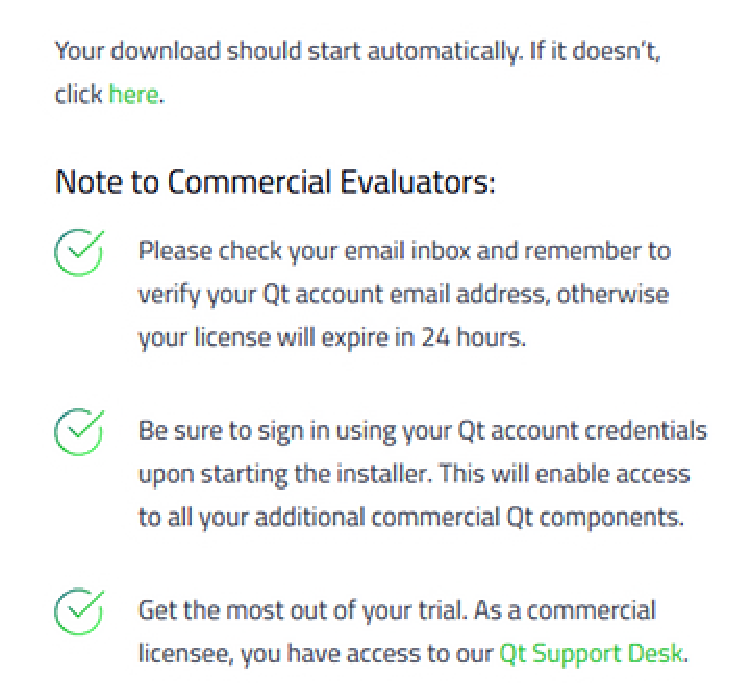
\includegraphics[width=8cm]{the_book_image/p000000.eps}} %图片路径
\caption{Qt在线安装包下载路径} %标题
\label{p000000} %索引
\end{figure}
%end图片

以管理员身份运行在线安装包,
选择安装路径时请不要选择包含空格和中文字符的路径。
虽然现代开发环境对于空格和中文字符支持良好,
但是,很多第三方辅助工具未必支持空格和中文字符。
包括本书自带的辅助工具也不保证支持空格和中文。

在Windows平台下,建议读者选择安装“MSVC 2017 64\hspace{0.05em}\rule[0.7ex]{0.4em}{0.65pt}\hspace{0.05em}bit”或以上版
或者
“MinGW 7.3.0 64\hspace{0.05em}\rule[0.7ex]{0.4em}{0.65pt}\hspace{0.05em}bit”或以上版本。
Qt选择5.12.0或以上版本。
安装的时候最好选择安装“Sources”、“Qt Charts”、“Qt WebEngine”以及
“Qt Debug Information Files”这些模块。
在“Tools”选项下组好安装“CDB”以及对应的“MinGW”。
本书建议最小安装如\figurename\ \ref{p000001}。
%begin图片
\begin{figure}[htb] %浮动体 here and top ...
%there must use marginnote ...
\marginnote{\setlength\fboxsep{2pt}\fbox{\footnotesize{\kaishu\figurename\,}\footnotesize{\ref{p000001}}}}\centering %中心对齐
\setlength\fboxsep{-1pt}\fbox{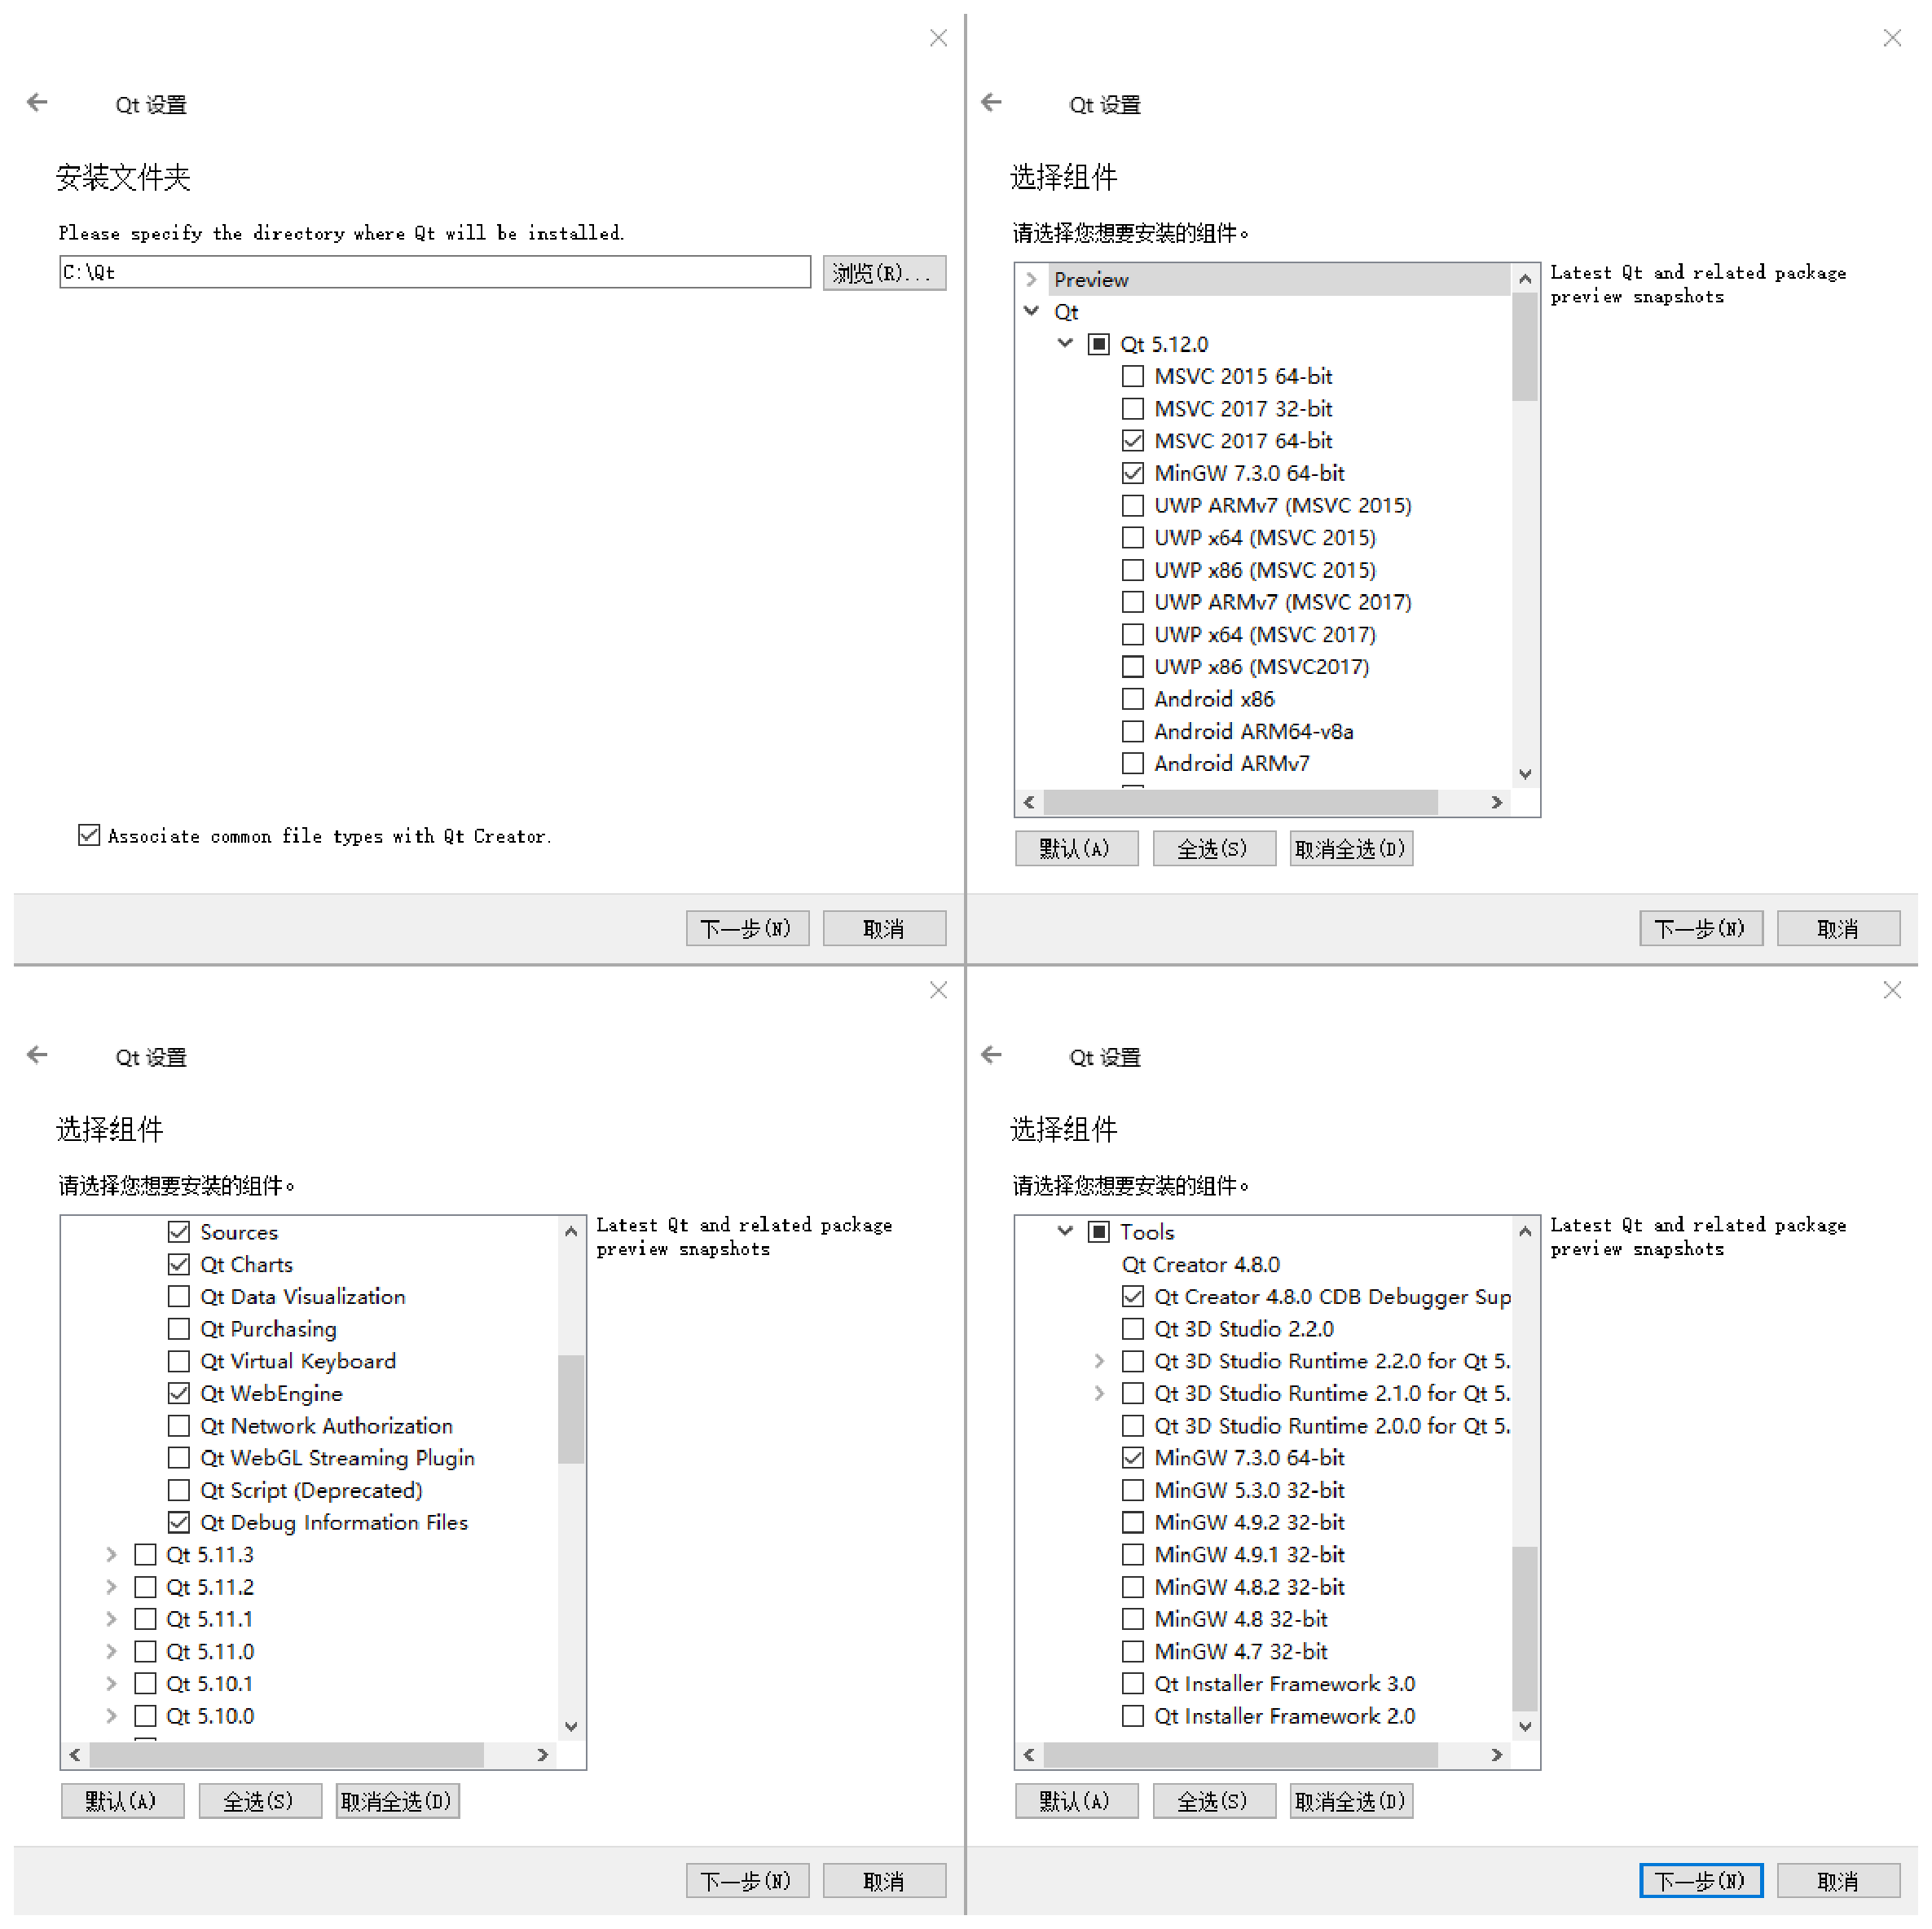
\includegraphics[width=0.95\textwidth]{the_book_image/p000001.eps}} %图片路径
\caption{Qt在线安装建议安装组件} %标题
\label{p000001} %索引
\end{figure}
%end图片


\FloatBarrier
\subsubsection{
在Windows平台下安装Boost
}\label{ss000210}

读者需要到Boost官网 \url{https://www.boost.org/
}下载最新Boost稳定版。解压缩,将“boost”文件夹复制到Qt Include路径。

比如,
用户的Qt Include路径为:
\begin{littlelongworld}
C:\textbackslash{}Qt\textbackslash{}Qt5.12.0\textbackslash{}5.12.0\textbackslash{}msvc2017\underline{\hspace{0.5em}}64\textbackslash{}include
\end{littlelongworld}
\hspace*{\parindent}复制完boost之后,
应当存在路径:
\begin{littlelongworld}
C:\textbackslash{}Qt\textbackslash{}Qt5.12.0\textbackslash{}5.12.0\textbackslash{}msvc2017\underline{\hspace{0.5em}}64\textbackslash{}include\textbackslash{}boost
\end{littlelongworld}
\hspace*{\parindent}当然,读者也可以采用“mklink”建立链接代替拷贝。

如果读者使用的是Visual Studio自带的编译器,则需要使用“Visual Studio命令提示符”运
行\commandnumbernameone\ \ref{command000002s02}。
并将编译结果的“\raisebox{-0.35ex}{\sourcefonttwo{}*}.lib”文件拷贝到Qt根目录下的lib文件夹,
将“\raisebox{-0.35ex}{\sourcefonttwo{}*}.dll”文件拷贝到Qt根目录下的bin文件夹。

\renewcommand\thelstnumber{\ifnum\value{lstnumber}>3{\ }\else{\arabic{lstnumber}}\fi}
%\begin{spacing}{1.0}
%\FloatBarrier
\refstepcounter{commandnumber}\label{command000002s02}    %增加命令行编号
\begin{thebookfilesourceonecommand}[escapeinside={(*@}{@*)},
caption=GoodLuck,
title=\commandnumbernameone \thecommandnumber
]
cd /D < Boost源代码路径 >
bootstrap.bat
bjam --build-type=complete
     --toolset=< MSVC版本比如:msvc-14.1 >
     address-model=64
     link=shared
     runtime-link=shared
     threading=multi(*@\marginpar[\hfill\setlength\fboxsep{2pt}\fbox{\footnotesize{\kaishu\parbox{1em}{\setlength{\baselineskip}{2pt}\commandnumbernameone}}\footnotesize{\thecommandnumber}}]{\setlength\fboxsep{2pt}\fbox{\footnotesize{\kaishu\parbox{1em}{\setlength{\baselineskip}{2pt}\commandnumbernameone}}\footnotesize{\thecommandnumber}}}@*)\end{thebookfilesourceonecommand}          %抄录环境
\addtocounter{lstlisting}{-1}   %sub lstlisting counter ...
%\end{spacing}

\renewcommand\thelstnumber{\arabic{lstnumber}}

之后,读者需要根据编译输出更新“QtQmlBook/msvc\underline{\hspace{0.5em}}boost.pri”文件。
如\filesourcenumbernameone\ \ref{f000041}
所示:
%\begin{spacing}{1.0}
\refstepcounter{filesourcenumber}\label{f000041}    %增加源代码编号
\FloatBarrier                                  %强制完成浮动体布局
\begin{thebookfilesourceone}[escapeinside={(*@}{@*)},
caption=GoodLuck,
title=\filesourcenumbernameone \thefilesourcenumber
,numbers=none]
CONFIG(debug,debug|release){
    LIBS += "boost_atomic-vc141-mt-gd-x64-1_68.lib"
    ……
else{
    LIBS += "boost_atomic-vc141-mt-x64-1_68.lib"
    ……
}(*@\marginpar[\hfill\setlength\fboxsep{2pt}\fbox{\footnotesize{\kaishu\parbox{1em}{\setlength{\baselineskip}{2pt}\filesourcenumbernameone}}\footnotesize{\thefilesourcenumber}}]{\setlength\fboxsep{2pt}\fbox{\footnotesize{\kaishu\parbox{1em}{\setlength{\baselineskip}{2pt}\filesourcenumbernameone}}\footnotesize{\thefilesourcenumber}}}@*)\end{thebookfilesourceone}          %抄录环境
\addtocounter{lstlisting}{-1}   %sub lstlisting counter ...
%\end{spacing}


如果读者使用的是MinGW环境,则需要使用“MinGW命令提示符”运
行\commandnumbernameone\ \ref{command000002s01}。
并将编译结果的“\raisebox{-0.35ex}{\sourcefonttwo{}*}.a”文件拷贝到Qt根目录下的lib文件夹,
将“\raisebox{-0.35ex}{\sourcefonttwo{}*}.dll”文件拷贝到Qt根目录下的bin文件夹。

\renewcommand\thelstnumber{\ifnum\value{lstnumber}>3{\ }\else{\arabic{lstnumber}}\fi}
%\begin{spacing}{1.0}
%\FloatBarrier
\refstepcounter{commandnumber}\label{command000002s01}    %增加命令行编号
\begin{thebookfilesourceonecommand}[escapeinside={(*@}{@*)},
caption=GoodLuck,
title=\commandnumbernameone \thecommandnumber
]
cd /D < Boost源代码路径 >
bootstrap.bat
bjam --build-type=complete
     --toolset=gcc
     address-model=64
     link=shared
     runtime-link=shared
     threading=multi(*@\marginpar[\hfill\setlength\fboxsep{2pt}\fbox{\footnotesize{\kaishu\parbox{1em}{\setlength{\baselineskip}{2pt}\commandnumbernameone}}\footnotesize{\thecommandnumber}}]{\setlength\fboxsep{2pt}\fbox{\footnotesize{\kaishu\parbox{1em}{\setlength{\baselineskip}{2pt}\commandnumbernameone}}\footnotesize{\thecommandnumber}}}@*)\end{thebookfilesourceonecommand}          %抄录环境
\addtocounter{lstlisting}{-1}   %sub lstlisting counter ...
%\end{spacing}

\renewcommand\thelstnumber{\arabic{lstnumber}}

之后,读者需要根据编译输出更新“QtQmlBook/mingw\underline{\hspace{0.5em}}boost.pri”文件。
如\filesourcenumbernameone\ \ref{f000040}
所示:
%\begin{spacing}{1.0}
\refstepcounter{filesourcenumber}\label{f000040}    %增加源代码编号
\FloatBarrier                                  %强制完成浮动体布局
\begin{thebookfilesourceone}[escapeinside={(*@}{@*)},
caption=GoodLuck,
title=\filesourcenumbernameone \thefilesourcenumber
,numbers=none]
CONFIG(debug,debug|release){
    LIBS += "libboost_atomic-mgw73-mt-d-x64-1_68.dll"
    ……
}else{
    LIBS += "libboost_atomic-mgw73-mt-x64-1_68.dll"
    ……
}(*@\marginpar[\hfill\setlength\fboxsep{2pt}\fbox{\footnotesize{\kaishu\parbox{1em}{\setlength{\baselineskip}{2pt}\filesourcenumbernameone}}\footnotesize{\thefilesourcenumber}}]{\setlength\fboxsep{2pt}\fbox{\footnotesize{\kaishu\parbox{1em}{\setlength{\baselineskip}{2pt}\filesourcenumbernameone}}\footnotesize{\thefilesourcenumber}}}@*)\end{thebookfilesourceone}          %抄录环境
\addtocounter{lstlisting}{-1}   %sub lstlisting counter ...
%\end{spacing}


\FloatBarrier
\subsubsection{
在Windows平台下MinGW配置jemalloc
}\label{ss000310}


%LD_PRELOAD
%由于Windows平台下不存在类似于Linux平台“LD_PRELOAD”这样可以动态
对于C{\sourcefonttwo{}+}{\sourcefonttwo{}+}来说,小对象的内存碎片问题向来很棘手。
一般而言,使用tcmalloc或jemalloc可以有效避免内存碎片问题。

在Linux平台或类似平台下,
可以使用“LD\underline{\hspace{0.5em}}PRELOAD”或类似的技术轻松的覆盖动态链接库中的函数。
因而,在Linux平台下,使用tcmalloc或jemalloc替换C库中的内存分配函数是简易的。

而在Windows平台下,
覆盖动态库中的函数相当复杂。
为了能够使得本书的示例代码不是玩具,
本书在Windows平台下使用jemalloc克服小对象内存碎片。

当使用MSVC编译器的时候,本书直接嵌入jemalloc源代码,
因而读者不必特别操心。
但是,当在Windows下使用MinGW编译器时,
读者需要自己静态编译jemalloc\footnote{
如果读者使用MinGW 7.3 64 bit版本的编译器,
本书已经将对应版本的jemalloc编译好了,
读者不需要再次编译。
}。
并将编译结果放置到:
\begin{littlelongworld}
QtQmlBook\textbackslash{}sstd\underline{\hspace{0.5em}}library\textbackslash{}memory\textbackslash{}libs
\end{littlelongworld}
文件夹下。
并将文件重命名为“jemalloc\underline{\hspace{0.5em}}win64\underline{\hspace{0.5em}}mingw\underline{\hspace{0.5em}}730.a”。
如果读者实在无法静态编译jemalloc,
读者可以找到:
\begin{littlelongworld}
QtQmlBook\textbackslash{}sstd\underline{\hspace{0.5em}}library\textbackslash{}\underline{\hspace{0.5em}}sstd\underline{\hspace{0.5em}}library\underline{\hspace{0.5em}}memory.pri
\end{littlelongworld}
并将此文件内容清空\footnote{
注意不要删除这个文件,而只是删除此文件内容。
}。


















%使用XeLaTeX编译
%版权所有,翻版必究
%本文件由程序自动生成,任何修改将被覆盖
%2019 年 01 月 23 日





%使用xelatex编译
%版权所有,翻版必究
%本文件由程序自动生成,任何修改将被覆盖
%2019 年 01 月 09 日




%

\FloatBarrier
\subsection{
在Linux平台下搭建开发环境
}\label{s000210}


Linux有众多发行版,
如果读者是首次在Linux平台下搭建Qt开发环境,建
议读者使用Ubuntu等使用者较多的版本。

\FloatBarrier
\subsubsection{
在Linux平台下安装Qt
}\label{ss000410}



如\commandnumbernameone\ \ref{command000000},所示:

\begin{itemize}
\item 第1行命令用于安装基本C{\sourcefonttwo{}+}{\sourcefonttwo{}+}开发环境;
\item 第2行命令用于安装OpenGL环境;
\end{itemize}

%\begin{spacing}{1.0}
%\FloatBarrier
\refstepcounter{commandnumber}\label{command000000}    %增加命令行编号
\begin{lstlisting}[escapeinside={(*@}{@*)},
caption=GoodLuck,
title=\commandnumbernameone\ \thecommandnumber
]
sudo apt-get install build-essential
sudo apt-get install libgl1-mesa-dev(*@\marginpar{\fbox{\footnotesize{\commandnumbernameone\ \thecommandnumber}}}@*)\end{lstlisting}          %抄录环境
%\end{spacing}


读者可以参照\ \ref{ss000110}
节相关内容下载最新的Qt开发包并安装,如\commandnumbernameone\ \ref{command000001}所示:

\begin{itemize}
\item 第1行命令用于赋予Qt安装包执行权限;
\item 第2行运行安装包;
\end{itemize}

%\begin{spacing}{1.0}
%\FloatBarrier
\refstepcounter{commandnumber}\label{command000001}    %增加命令行编号
\begin{lstlisting}[escapeinside={(*@}{@*)},
caption=GoodLuck,
title=\commandnumbernameone\ \thecommandnumber
]
chmod +x qt-opensource-linux-x64-5.12.0.run
./qt-opensource-linux-x64-5.12.0.run(*@\marginpar{\fbox{\footnotesize{\commandnumbernameone\ \thecommandnumber}}}@*)\end{lstlisting}          %抄录环境
%\end{spacing}


在不同Linux发行版本这些命令有所不同,
即使是同一发行版本,
随着时间推移命令也会有所变化。

读者可以访问\ \url{https://wiki.qt.io/Main}
获得更加详细的帮助。




\FloatBarrier
\subsubsection{
在Linux平台下安装Boost
}\label{ss000510}



在Linux下安装Boost极其简单,只需要执
行\commandnumbernameone\ \ref{command000002}即可。

%\begin{spacing}{1.0}
%\FloatBarrier
\refstepcounter{commandnumber}\label{command000002}    %增加命令行编号
\begin{lstlisting}[escapeinside={(*@}{@*)},
caption=GoodLuck,
title=\commandnumbernameone\ \thecommandnumber
]
sudo apt-get install libboost-all-dev(*@\marginpar{\fbox{\footnotesize{\commandnumbernameone\ \thecommandnumber}}}@*)\end{lstlisting}          %抄录环境
%\end{spacing}



%不过相对于Windows平台 ,
%Linux这种直接使用全局库
%反而比Windows下直接拷贝
%隐含了更多问题。










%使用xelatex编译
%版权所有,翻版必究
%本文件由程序自动生成,任何修改将被覆盖
%2019 年 01 月 09 日








% ______all_key_words
% the_book_chapter the_book_subsection the_book_subsubsection
% the_book_section the_book_image the_book_table
% the_book_file the_book_tree_file the_book_command_file
% littlelongworld tabbing ref
% figurename tablename filesourcenumbernameone
% treeindexnumbernameone commandnumbernameone footnote 
% item itemize comment textbullet
% \hspace*{\parindent}







%使用XeLaTeX编译
%版权所有,翻版必究
%本文件由程序自动生成,任何修改将被覆盖
%2019 年 01 月 23 日




%使用xelatex编译
%版权所有,翻版必究
%本文件由程序自动生成,任何修改将被覆盖





%


\subsection{
qmake入门
}\label{s100310}


qmake类似于cmake,但qmake比cmake更加简洁清晰。
如果读者希望写一个跨平台的库的话,
或许cmake是比qmake更加优异的选择。
但读者明确是写一个特定的应用程序的话,
qmake就比cmake优秀的多。
qmake比cmake确实功能较少,
但从另一个角度,
qmake比cmake更加专注。
通过本节,
读者会发现只需要学习可怜的一点内容,
就可以使用qmake搭建出复杂的程序架构。

%%%%%%%%%%%%%%%%%%%%%%%%%%%%%%%%%%%%%%%%%%%%%%%%%%%%%%%%

\subsubsection{
使用qmake构建Hellow World!
}\label{ss000610}

读者新建一个目录\footnote{
本书所有目录都要求不包含空格和中文,以后不再赘述。
},
在此文件夹下新建一个“hellow\underline{\hspace{0.5em}}world.pro”文件,输入文件内容如
\lstlistingname\ \ref{f000002}。
在此文件夹下建立“main.cpp”文件,输入内容如
\lstlistingname\ \ref{f000003}。

\begin{lstlisting}[label=f000002,
caption=GoodLuck,
title=\lstlistingname\ \thelstlisting
]
QT -= gui
QT -= core

CONFIG += console

CONFIG(debug,debug|release){
    TARGET = hellow_word_debug
}else{
    TARGET = hellow_word
}

TEMPLATE = app

win32-msvc*{
    QMAKE_CXXFLAGS += /std:c++latest
}else{
    CONFIG += c++17
}

SOURCES += $$PWD/main.cpp
DESTDIR =  $$PWD

DEFINES *= NUMBER=1
DEFINES *= HELLOW=\\\"Hellow\\\"
DEFINES += QT_DEPRECATED_WARNINGS
\end{lstlisting}          %抄录环境

\begin{lstlisting}[label=f000003,
caption=GoodLuck,
title=\lstlistingname\ \thelstlisting
]
#include <iostream>

int main(int , char **) {
    if constexpr(NUMBER) {
        std::cout << HELLOW " World! "
                  << std::endl;
    }
}
\end{lstlisting}          %抄录环境


使用QtCreator打开“hellow\underline{\hspace{0.5em}}world.pro”,
运行此项目。

现在来分析一下\lstlistingname\ \ref{f000002}:
\begin{itemize}
\item 第1\~{}2行表示不使用Qt库;
\item 第4行表示这是一个控制台应用程序;
\item 第6\~{}10行表示在debug模式下输出目标名称是“hellow\underline{\hspace{0.5em}}world\underline{\hspace{0.5em}}debug”,
在release模式下输出目标名称是“hellow\underline{\hspace{0.5em}}world”;
\item 第12行表示输出的是一个应用程序;
\item 第14\~{}18行表示使用C++17标准;
\item 第20行将“main.cpp”加入编译过程;
\item 第21行规定输出目录就是当前“pro”文件所在目录;
\item 第23行定义了一个叫“NUMBER”的宏,宏的值是一个数字;
\item 第24行定义了一个叫“HELLOW”的宏,宏的值是一个字符串;
\item 第25行定义了一个叫“QT\underline{\hspace{0.5em}}DEPRECATED\underline{\hspace{0.5em}}WARNINGS”的宏,这个宏没有定义值;
\end{itemize}

不难发现qmake的语法十分简单:
\begin{itemize}
\item “=”代表赋值;
\item “+=”代表向对象中增加元素;
\item “-=”代表从对象中删除元素;
\item “*=”代表如果对象中不存在则加入元素否则忽略;
\item “\$\$”代表将对象转换为字面值;
\item “SOURCES”代表需要编译的C/C++源代码对象;
\item “HEADERS”代表C/C++头文件对象;
\item “DEFINES”代表C/C++宏对象;
\item “TARGET”代表输出对象名称;
\item “CONFIG”用来加入和检查Qt中预定义的编译选项;
\item “QMAKE\underline{\hspace{0.5em}}CXXFLAGS”代表qmake生成MakeFile时需要加入的编译期参数;
\item “TEMPLATE”决定此项目的模板类型,本案例是使用应用程序模板(app)后续章节会介绍更多模板;
\end{itemize}


%%%%%%%%%%%%%%%%%%%%%%%%%%%%%%%%%%%%%%%%%%%%%%%%%%%%%%%%

\subsubsection{
使用qmake创建动态链接库
}\label{ss000710}


%%%%%%%%%%%%%%%%%%%%%%%%%%%%%%%%%%%%%%%%%%%%%%%%%%%%%%%%

\subsubsection{
qmake高级用法
}\label{ss000810}


\stepcounter{treeIndexNumber}%增加目录树编号
\begin{lstlisting}[label=d000000,
numbers=none,
title=\theTreeIndexNumber
]
.
├── advance_use_qmake.pro
├── after_run
│   ├── after_run.pro
│   └── main.cpp
├── before_run
│   ├── before_run.pro
│   └── main.cpp
├── new_moc
│   ├── main.cpp
│   └── new_moc.pro
└── the_run
    ├── main.cpp
    ├── test1.hpp
    ├── test2.hpp
    └── the_run.pro
\end{lstlisting}          %抄录环境


\begin{lstlisting}[label=f000004,
caption=GoodLuck,
title=\lstlistingname\ \thelstlisting
]
TEMPLATE = subdirs

CONFIG += ordered

new_moc.file = $$PWD/new_moc/new_moc.pro
SUBDIRS += new_moc

before_run.file = $$PWD/before_run/before_run.pro
SUBDIRS += before_run

after_run.file = $$PWD/after_run/after_run.pro
SUBDIRS += after_run

the_run.file = $$PWD/the_run/the_run.pro
SUBDIRS += the_run
\end{lstlisting}          %抄录环境

\begin{lstlisting}[label=f000005,
caption=GoodLuck,
title=\lstlistingname\ \thelstlisting
]
QT -= gui
QT -= core

CONFIG += console

CONFIG(debug,debug|release){
    TARGET = the_run_debug
}else{
    TARGET = the_run
}

TEMPLATE = app

win32-msvc*{
    QMAKE_CXXFLAGS += /std:c++latest
}else{
    CONFIG += c++17
    LIBS += -lstdc++fs
}

SOURCES += $$PWD/main.cpp
DESTDIR =  $$PWD/../bin

DEFINES += QT_DEPRECATED_WARNINGS

#when before build new_moc will call ...
new_moc.dependency_type = TYPE_C
new_moc.variable_out = SOURCES
new_moc.output  = moc_new_${QMAKE_FILE_BASE}.cpp
CONFIG(debug,debug|release){
new_moc.commands = \
$${DESTDIR}/new_moc_debug ${QMAKE_FILE_NAME} ${QMAKE_FILE_OUT}
}else{
new_moc.commands = \
$${DESTDIR}/new_moc ${QMAKE_FILE_NAME} ${QMAKE_FILE_OUT}
}
NEW_MOC_HEADERS = test2.hpp test1.hpp
new_moc.input = NEW_MOC_HEADERS
QMAKE_EXTRA_COMPILERS += new_moc

#when link started before_run will call ...
CONFIG(debug,debug|release){
    QMAKE_PRE_LINK += $${DESTDIR}/before_run_debug $$PWD
}else{
    QMAKE_PRE_LINK += $${DESTDIR}/before_run $$PWD
}
export(QMAKE_PRE_LINK)

#when link finished after_run will call ...
CONFIG(debug,debug|release){
    QMAKE_POST_LINK += $${DESTDIR}/after_run_debug $$PWD
}else{
    QMAKE_POST_LINK += $${DESTDIR}/after_run $$PWD
}
export(QMAKE_POST_LINK)
\end{lstlisting}          %抄录环境

\begin{lstlisting}[label=f00000a,
caption=GoodLuck,
title=\lstlistingname\ \thelstlisting
]
#if __has_include(<filesystem>)
#include <filesystem>
namespace fs = std::filesystem;
#else
#include <experimental/filesystem>
namespace fs = std::experimental::filesystem;
#endif
#include <iostream>

int main(int, char **) {
    std::cout << "the_run" << std::endl;
    return 0;
}
\end{lstlisting}          %抄录环境

\begin{lstlisting}[label=f000006,
caption=GoodLuck,
title=\lstlistingname\ \thelstlisting
]
QT -= gui
QT -= core

CONFIG += console

CONFIG(debug,debug|release){
    TARGET = after_run_debug
}else{
    TARGET = after_run
}

TEMPLATE = app

win32-msvc*{
    QMAKE_CXXFLAGS += /std:c++latest
}else{
    CONFIG += c++17
    LIBS += -lstdc++fs
}

SOURCES += $$PWD/main.cpp
DESTDIR =  $$PWD/../bin

DEFINES += QT_DEPRECATED_WARNINGS
\end{lstlisting}          %抄录环境

\begin{lstlisting}[label=f000007,
caption=GoodLuck,
title=\lstlistingname\ \thelstlisting
]
#if __has_include(<filesystem>)
#include <filesystem>
namespace fs = std::filesystem;
#else
#include <experimental/filesystem>
namespace fs = std::experimental::filesystem;
#endif

#include <iostream>
#include <fstream>
#include <chrono>

class OStream :public std::ofstream {
    using Super = std::ofstream;
public:
    template<typename T,
        typename = std::enable_if_t<
        std::is_constructible_v<Super, T && > > >
        inline OStream(T && arg) :
        Super(std::forward<T>(arg)) {
    }
    template<typename T,
        typename = void,
        typename = std::enable_if_t<
        !std::is_constructible_v<Super, T && > > >
        inline OStream(T && arg) :
        Super(std::forward<T>(arg).string()) {
    }
};

int main(int argc, char ** argv) {
    std::cout << "before_run : "
        << argc << std::endl;
    if (argc < 2) {
        return -1;
    }
    fs::path varPath{ argv[1] };
    OStream stream{ varPath / "after_run.txt" };
    stream << std::chrono::
        high_resolution_clock::now()
        .time_since_epoch().count();
    stream << std::endl;
    return 0;
}
\end{lstlisting}          %抄录环境

\begin{lstlisting}[label=f000008,
caption=GoodLuck,
title=\lstlistingname\ \thelstlisting
]
QT -= gui
QT -= core

CONFIG += console

CONFIG(debug,debug|release){
    TARGET = before_run_debug
}else{
    TARGET = before_run
}

TEMPLATE = app

win32-msvc*{
    QMAKE_CXXFLAGS += /std:c++latest
}else{
    CONFIG += c++17
    LIBS += -lstdc++fs
}

SOURCES += $$PWD/main.cpp
DESTDIR =  $$PWD/../bin

DEFINES += QT_DEPRECATED_WARNINGS
\end{lstlisting}          %抄录环境

\begin{lstlisting}[label=f000009,
caption=GoodLuck,
title=\lstlistingname\ \thelstlisting
]
#if __has_include(<filesystem>)
#include <filesystem>
namespace fs = std::filesystem;
#else
#include <experimental/filesystem>
namespace fs = std::experimental::filesystem;
#endif

#include <iostream>
#include <fstream>
#include <chrono>

class OStream :public std::ofstream {
    using Super = std::ofstream;
public:
    template<typename T,
        typename = std::enable_if_t<
        std::is_constructible_v<Super, T && > > >
        inline OStream(T && arg) :
        Super(std::forward<T>(arg)) {
    }
    template<typename T,
        typename = void,
        typename = std::enable_if_t<
        !std::is_constructible_v<Super, T && > > >
        inline OStream(T && arg) :
        Super(std::forward<T>(arg).string()) {
    }
};

int main(int argc, char ** argv) {
    std::cout << "before_run : "
        << argc << std::endl;
    if (argc < 2) {
        return -1;
    }
    fs::path varPath{ argv[1] };
    OStream stream{ varPath / "before_run.txt" };
    stream << std::chrono::
        high_resolution_clock::now()
        .time_since_epoch().count();
    stream << std::endl;
    return 0;
}
\end{lstlisting}          %抄录环境

\begin{lstlisting}[label=f00000b,
caption=GoodLuck,
title=\lstlistingname\ \thelstlisting
]
QT -= gui
QT -= core

CONFIG += console

CONFIG(debug,debug|release){
    TARGET = new_moc_debug
}else{
    TARGET = new_moc
}

TEMPLATE = app

win32-msvc*{
    QMAKE_CXXFLAGS += /std:c++latest
}else{
    CONFIG += c++17
    LIBS += -lstdc++fs
}

SOURCES += $$PWD/main.cpp
DESTDIR =  $$PWD/../bin

DEFINES += QT_DEPRECATED_WARNINGS
\end{lstlisting}          %抄录环境

\begin{lstlisting}[label=f00000c,
caption=GoodLuck,
title=\lstlistingname\ \thelstlisting
]
#include <iostream>
#include <fstream>

#if __has_include(<filesystem>)
#include <filesystem>
namespace fs = std::filesystem;
#else
#include <experimental/filesystem>
namespace fs = std::experimental::filesystem;
#endif

int main(int argc, char ** argv) {
    std::cout << "new_moc : "
        << argc << std::endl;
    if (argc < 3) {
        return -1;
    }
    std::ifstream varInput{ argv[1] };
    std::ofstream varOutput{ argv[2] };
    varOutput << "/*****************************/";
    varOutput << std::endl;
    varOutput << "#include \"";
    varOutput << argv[1];
    varOutput << "\"";
    varOutput << std::endl;
    varOutput << u8R"(inline static int a = [](){
               std::cout << "Good Luck!" <<std::endl;
               return 12;
               }() ; )";
    varOutput << std::endl;
    return 0;
}
\end{lstlisting}          %抄录环境


%%%%%%%%%%%%%%%%%%%%%%%%%%%%%%%%%%%%%%%%%%%%%%%%%%%%%%%%

\subsubsection{
qmake杂项
}\label{ss000910}










%使用xelatex编译
%版权所有,翻版必究
%本文件由程序自动生成,任何修改将被覆盖




%使用xelatex编译
%版权所有,翻版必究
%本文件由程序自动生成,任何修改将被覆盖




%


\subsection{
第一个程序
}\label{s100210}



读者可以使用Qt Creator打开“QtQmlBook.pro”。
在Windows平台下,读者
也可以修改“build\underline{\hspace{0.5em}}msvc.bat”,从而使用Visual Studio。

如\lstlistingname\ \ref{f000018} :


%\begin{spacing}{1.0}
\begin{lstlisting}[label=f000018,
caption=GoodLuck,
title=\lstlistingname\ \thelstlisting
]
call "C:/Qt/Qt5.12.0/5.12.0/msvc2017_64/bin/qtenv2.bat"
cd /D "E:/QtQmlBookMsvc"
qmake -r -tp vc "E:/QtQmlBook/QtQmlBook.pro"
qmake -r -tp vc "E:/QtQmlBook/QtQmlMultimedia.pro"
qmake -r -tp vc "E:/QtQmlBook/QtQmlBookTest.pro"
qmake -r -tp vc "E:/QtQmlBook/TheBook/TheBook.pro"
cmd
\end{lstlisting}          %抄录环境
%\end{spacing}



\begin{itemize}

\item 第1行用于设置Qt运行环境;
\item 第2行用于设置Visual Studio工程文件输出目录;
\item 第3\raisebox{0.16ex}{\sourcefonttwo\~{}}6行用于指明将哪些qmake项目转为Visual Studio项目;

\end{itemize}





































%使用xelatex编译
%版权所有,翻版必究
%本文件由程序自动生成,任何修改将被覆盖





%使用xelatex编译
%版权所有,翻版必究
%本文件由程序自动生成,任何修改将被覆盖
%2019 年 01 月 09 日





\FloatBarrier
\section{
你好世界!
}\label{s100410}


%begin图片
\begin{figure}[htb] %浮动体 here and top ...
%there must use marginnote not use marginpar ...
\marginnote{\setlength\fboxsep{2pt}\fbox{\footnotesize{\kaishu\figurename\,}\footnotesize{\ref{p000006}}}}\centering %中心对齐
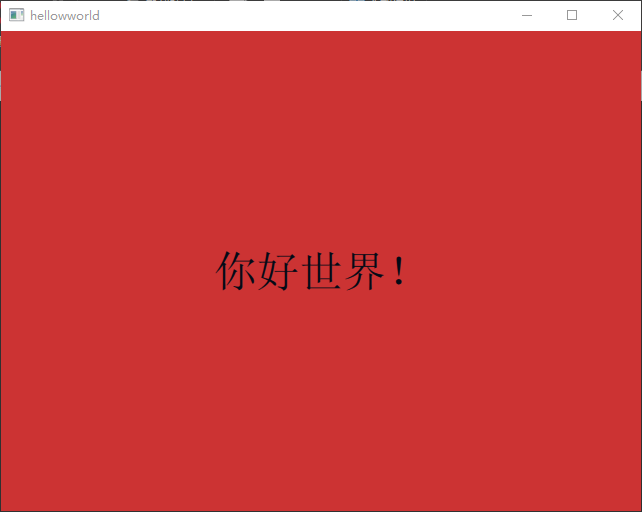
\includegraphics[width=0.95\textwidth]{../chapter01/hellowworld/the_app.png} %图片路径
\caption{你好世界!} %标题
\label{p000006} %索引
\end{figure}
%end图片


绝大多数介绍计算机语言的书籍都有一
个“Hellow World!”的案例,本书也不能免俗。

本章的C{\sourcefonttwo{}+}{\sourcefonttwo{}+}代码
如\lstlistingname\ \ref{f000030}:

%\begin{spacing}{1.0}
\FloatBarrier
\begin{thebookfilesourceone}[escapeinside={(*@}{@*)},
label=f000030,
caption=GoodLuck,
title=\lstlistingname \thelstlisting
]
#include <sstd_qt_and_qml_library.hpp>

int main(int argc, char ** argv) {

    /*初始化程序*/
    auto varApp = sstd_make_unique< sstd::Application >(argc, argv);
    /*初始化Qml/Quick引擎*/
    auto varWindow = sstd_make_unique< sstd::DefaultRoowWindow >();
    {
        /*获得Qml文件绝对路径*/
        auto varFullFileName = sstd::getLocalFileFullPath(
            QStringLiteral("myqml/hellowworld/main.qml"));
        /*加载Qml文件*/
        varWindow->load(varFullFileName);
        /*检查并报错*/
        if (varWindow->status() != sstd::LoadState::Ready) {
            qWarning() <<
                       QStringLiteral("can not load : ")
                       << varFullFileName;
            return -1;
        }
    }
    varWindow->show();

    return varApp->exec();

}(*@\marginpar[\hfill\setlength\fboxsep{2pt}\fbox{\footnotesize{\kaishu\parbox{1em}{\setlength{\baselineskip}{2pt}\lstlistingname}}\footnotesize{\thelstlisting}}]{\setlength\fboxsep{2pt}\fbox{\footnotesize{\kaishu\parbox{1em}{\setlength{\baselineskip}{2pt}\lstlistingname}}\footnotesize{\thelstlisting}}}@*)\end{thebookfilesourceone}          %抄录环境
%\end{spacing}
%main.cpp

本书将大量的程序细节隐藏到了“sstd\underline{\hspace{0.5em}}qt\underline{\hspace{0.5em}}and\underline{\hspace{0.5em}}qml\underline{\hspace{0.5em}}library”库里面。

\begin{itemize}
\item sstd::Application用于构造QApplication,
并初始化Qt Quick运行所需的参数;
\item sstd::DefaultRoowWindow在Debug
模式下继承自QQuickWidget,在Release模式下继承自QQuickView;
\item sstd::getLocalFileFullPath在
Debug模式以当前文件目录作为根目录,在Release模式下以应用程序
目录作为根目录;
\end{itemize}

本书以后章节的“main.cpp”都大同小异,以后不再赘述。


“main.qml”如\lstlistingname\ \ref{f000031}
所示:

%\begin{spacing}{1.0}
\FloatBarrier
\begin{thebookfilesourceone}[escapeinside={(*@}{@*)},
label=f000031,
caption=GoodLuck,
title=\lstlistingname \thelstlisting
]
/*main.qml*/
import QtQuick 2.9
import "main_private" as MainPrivate

Rectangle {

    width: 640
    height: 480
    color: Qt.rgba(0.8, 0.8, 0.8, 1)

    MainPrivate.MainText {
        z: 1
        anchors.fill: parent
    } /*~MainText*/

    MainPrivate.MainRectangle {
        z: 0
        anchors.fill: parent
    } /*~MainRectangle*/
} /*~Rectangle*/(*@\marginpar[\hfill\setlength\fboxsep{2pt}\fbox{\footnotesize{\kaishu\parbox{1em}{\setlength{\baselineskip}{2pt}\lstlistingname}}\footnotesize{\thelstlisting}}]{\setlength\fboxsep{2pt}\fbox{\footnotesize{\kaishu\parbox{1em}{\setlength{\baselineskip}{2pt}\lstlistingname}}\footnotesize{\thelstlisting}}}@*)\end{thebookfilesourceone}          %抄录环境
%\end{spacing}
%main.qml

\begin{itemize}

\item 第3行展示了如何引入其他目录的Qml文件。
其语法如\lstlistingname\ \ref{f000034}
所示:

%\begin{spacing}{1.0}
\FloatBarrier
\begin{thebookfilesourceone}[escapeinside={(*@}{@*)},
label=f000034,
caption=GoodLuck,
title=\lstlistingname \thelstlisting
]
import "ResourceURL" as Qualifier(*@\marginpar[\hfill\setlength\fboxsep{2pt}\fbox{\footnotesize{\kaishu\parbox{1em}{\setlength{\baselineskip}{2pt}\lstlistingname}}\footnotesize{\thelstlisting}}]{\setlength\fboxsep{2pt}\fbox{\footnotesize{\kaishu\parbox{1em}{\setlength{\baselineskip}{2pt}\lstlistingname}}\footnotesize{\thelstlisting}}}@*)\end{thebookfilesourceone}          %抄录环境
%\end{spacing}
%1.txt

\item 第5行定义了一个Rectangle:

%%%%%%%%%%%%%%%%%%%%%%%%%%%%%%%%%%%%%%%%%%%%%%%%%%

\begin{itemize}
\item 第7行定义了Rectangle的宽度;
\item 第8行定义了Rectangle的高度;
\item 第9行定义了Rectangle的颜色;
\end{itemize}

\item 第11\raisebox{0.16ex}{\sourcefonttwo\~{}}19行定义了两个子对象。
和Qt Widgets一样,子对象在父对象之上。兄弟对象之间的关系是,
后出现的对象在先出现的对象之上。
也可以调整z属性调整兄弟对象的上下关系。

读者可以尝试注释掉第12行和17行观察程序输出结果。

%%%%%%%%%%%%%%%%%%%%%%%%%%%%%%%%%%%%%%%%%%%%%%%%%%

\item 第13行和第18行使用“anchors”确保子对象完全覆盖父对象。

\end{itemize}

“MainRectangle.qml”如\lstlistingname\ \ref{f000032}
所示:
%\begin{spacing}{1.0}
\FloatBarrier
\begin{thebookfilesourceone}[escapeinside={(*@}{@*)},
label=f000032,
caption=GoodLuck,
title=\lstlistingname \thelstlisting
]
/*main_private/MainRectangle.qml*/
import QtQuick 2.9

Rectangle {
    color: Qt.rgba(0.8, 0.2, 0.2, 1)
}(*@\marginpar[\hfill\setlength\fboxsep{2pt}\fbox{\footnotesize{\kaishu\parbox{1em}{\setlength{\baselineskip}{2pt}\lstlistingname}}\footnotesize{\thelstlisting}}]{\setlength\fboxsep{2pt}\fbox{\footnotesize{\kaishu\parbox{1em}{\setlength{\baselineskip}{2pt}\lstlistingname}}\footnotesize{\thelstlisting}}}@*)\end{thebookfilesourceone}          %抄录环境
%\end{spacing}
%MainRectangle.qml

Qml是一门大小写敏感的计算机语言。
读者使用import命令引入Qml定义的对象时,文件名必须以大写开头;
而引入JavaScript文件时,
文件名应当以小写开头。

“MainText.qml”如\lstlistingname\ \ref{f000033}
所示:

%\begin{spacing}{1.0}
\FloatBarrier
\begin{thebookfilesourceone}[escapeinside={(*@}{@*)},
label=f000033,
caption=GoodLuck,
title=\lstlistingname \thelstlisting
]
/*main_private/MainText.qml*/
import QtQuick 2.9

Text {
    text: qsTr("你好世界!")
    color: Qt.rgba(Math.random() / 10, Math.random() / 10,
                   Math.random() / 10, 1)
    font.pointSize: 32
    verticalAlignment: Text.AlignVCenter
    horizontalAlignment: Text.AlignHCenter
}(*@\marginpar[\hfill\setlength\fboxsep{2pt}\fbox{\footnotesize{\kaishu\parbox{1em}{\setlength{\baselineskip}{2pt}\lstlistingname}}\footnotesize{\thelstlisting}}]{\setlength\fboxsep{2pt}\fbox{\footnotesize{\kaishu\parbox{1em}{\setlength{\baselineskip}{2pt}\lstlistingname}}\footnotesize{\thelstlisting}}}@*)\end{thebookfilesourceone}          %抄录环境
%\end{spacing}
%MainText.qml

\begin{itemize}

\item 第5行展示了如何在Qml中实现国际化,读者只需要用
qsTr包装字符串即可;
\item 第6\raisebox{0.16ex}{\sourcefonttwo\~{}}7行展示了可以在Qml中直接使用JavaScript;


\end{itemize}










%使用xelatex编译
%版权所有,翻版必究
%本文件由程序自动生成,任何修改将被覆盖
%2019 年 01 月 09 日





%使用XeLaTeX编译
%版权所有,翻版必究
%本文件由程序自动生成,任何修改将被覆盖
%2019 年 01 月 23 日




\FloatBarrier
\section{
初识Qt Quick控件
}\label{s100510}


%begin图片
\begin{figure}[htb] %浮动体 here and top ...
%there must use marginnote ...
\marginnote{\setlength\fboxsep{2pt}\fbox{\footnotesize{\kaishu\figurename\,}\footnotesize{\ref{p000007}}}}\centering %中心对齐
\setlength\fboxsep{0pt}\fcolorbox[rgb]{0,0,0}{0.97,0.98,0.99}{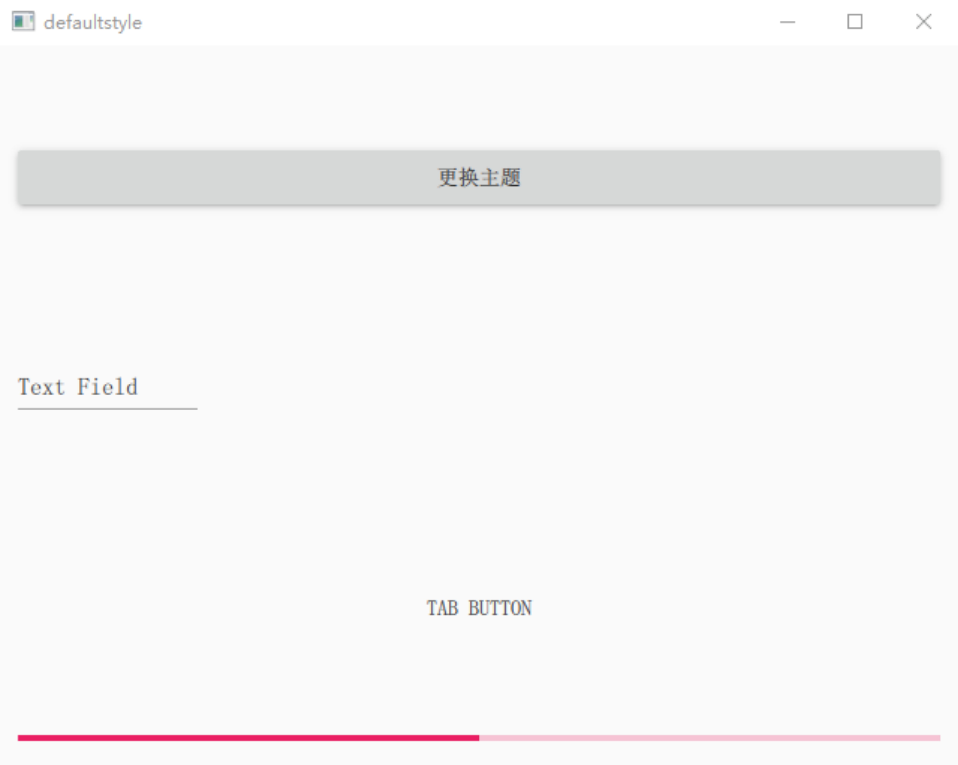
\includegraphics[width=0.95\textwidth]{the_book_image/p000007.pdf}} %图片路径
\caption{Qt Quick控件及样式!} %标题
\label{p000007} %索引
\end{figure}
%end图片


Qt Quick Controls 2 自Qt 5.7引入。

本书不加特别说明,提到Qt Quick Controls就是指
Qt Quick Controls 2。

Qt Quick Controls 1更多的是沿用传统桌面
的设计风格;而
Qt Quick Controls 2更加现代化并更适用于
移动设备。
并且,Qt Quick Controls 2对于主题和样式
提供了专门的语法支持。

基于这些语法,读者可以轻松的实现样式、内容和结构分离。
即使读者不想在样式上太花费心思,Qt Quick Controls 2也
默认提供了数个艺术级的样式模板。

除了维护老项目,
没有什么理由不采用Qt Quick Controls 2。

本项目的“main.qml”如\filesourcenumbernameone\ \ref{f000035}
所示:

%\begin{spacing}{1.0}
\refstepcounter{filesourcenumber}\label{f000035}    %增加源代码编号
\FloatBarrier                                  %强制完成浮动体布局
\begin{thebookfilesourceone}[escapeinside={(*@}{@*)},
caption=GoodLuck,
title=\filesourcenumbernameone \thefilesourcenumber
]
/*defaultstyle/main.qml*/
import QtQuick 2.9
import QtQuick.Controls 2.3
import QtQuick.Layouts 1.3
import QtQuick.Controls.Material 2.12

Pane {

    id : idRoot
    width: 640;
    height: 480;

    function changeTheme(){
        if(idRoot.Material.theme === Material.Dark ){
            idRoot.Material.theme = Material.Light;
        }else{
            idRoot.Material.theme = Material.Dark;
        }
    }

    ColumnLayout {
        id: idColumn
        anchors.fill: parent

        Button {
            id: idButton
            text: qsTr("更换主题")
            Layout.fillWidth : true
            onClicked: {
                idRoot.changeTheme();
            }
        }

        TextField {
            id: idTextField
            text: qsTr("Text Field")
            Layout.fillWidth : true
        }

        TabButton {
            id: idTabButton
            text: qsTr("Tab Button")
            Layout.fillWidth : true
        }

        ProgressBar {
            id: idProgressBar
            value: 0.5
            Layout.fillWidth : true
        }

    }

}/*~Pane*/(*@\marginpar[\hfill\setlength\fboxsep{2pt}\fbox{\footnotesize{\kaishu\parbox{1em}{\setlength{\baselineskip}{2pt}\filesourcenumbernameone}}\footnotesize{\thefilesourcenumber}}]{\setlength\fboxsep{2pt}\fbox{\footnotesize{\kaishu\parbox{1em}{\setlength{\baselineskip}{2pt}\filesourcenumbernameone}}\footnotesize{\thefilesourcenumber}}}@*)\end{thebookfilesourceone}          %抄录环境
\addtocounter{lstlisting}{-1}   %sub lstlisting counter ...
%\end{spacing}
%main.qml

\begin{itemize}
\item 第21行展示了如何使用Layout;
\item 第28行、第37行、第43行、第49行
展示了使用关联属性\footnote{
Attached Properties。
};
\item 第29\raisebox{0.16ex}{\sourcefonttwo\~{}}31行展示了如何关联一个Qml信号到一个
JavaScript函数;%……
\item 第13\raisebox{0.16ex}{\sourcefonttwo\~{}}19行展示了如何在一个Qml对象里面
使用JavaScript定义
一个槽函数;
\end{itemize}

本案例演示了如何使用Qt Quick Control自带的“Material”样式。

要使用Qt Quick Control自带的样式,需要在QApplication
构造之前调用如\filesourcenumbernameone\ \ref{f000037}
所示的C{\sourcefonttwo{}+}{\sourcefonttwo{}+}代码,以载入配置文件。

%\begin{spacing}{1.0}
\refstepcounter{filesourcenumber}\label{f000037}    %增加源代码编号
\FloatBarrier                                  %强制完成浮动体布局
\begin{thebookfilesourceone}[escapeinside={(*@}{@*)},
caption=GoodLuck,
title=\filesourcenumbernameone \thefilesourcenumber
]
::qputenv("QT_QUICK_CONTROLS_CONF","defaultstyle_qtquickcontrols2.conf");(*@\marginpar[\hfill\setlength\fboxsep{2pt}\fbox{\footnotesize{\kaishu\parbox{1em}{\setlength{\baselineskip}{2pt}\filesourcenumbernameone}}\footnotesize{\thefilesourcenumber}}]{\setlength\fboxsep{2pt}\fbox{\footnotesize{\kaishu\parbox{1em}{\setlength{\baselineskip}{2pt}\filesourcenumbernameone}}\footnotesize{\thefilesourcenumber}}}@*)\end{thebookfilesourceone}          %抄录环境
\addtocounter{lstlisting}{-1}   %sub lstlisting counter ...
%\end{spacing}


配置文件内容如\filesourcenumbernameone\ \ref{f000036}
所示:
%\begin{spacing}{1.0}
\refstepcounter{filesourcenumber}\label{f000036}    %增加源代码编号
\FloatBarrier                                  %强制完成浮动体布局
\begin{thebookfilesourceone}[escapeinside={(*@}{@*)},
caption=GoodLuck,
title=\filesourcenumbernameone \thefilesourcenumber
]
[Controls]
Style=Material
FallbackStyle=Material

[Material]
Theme=Dark(*@\marginpar[\hfill\setlength\fboxsep{2pt}\fbox{\footnotesize{\kaishu\parbox{1em}{\setlength{\baselineskip}{2pt}\filesourcenumbernameone}}\footnotesize{\thefilesourcenumber}}]{\setlength\fboxsep{2pt}\fbox{\footnotesize{\kaishu\parbox{1em}{\setlength{\baselineskip}{2pt}\filesourcenumbernameone}}\footnotesize{\thefilesourcenumber}}}@*)\end{thebookfilesourceone}          %抄录环境
\addtocounter{lstlisting}{-1}   %sub lstlisting counter ...
%\end{spacing}
%defaultstyle_qtquickcontrols2.conf

Qt Quick Control的样式具有继承性。

子控件的样式与父控件一致,
只需要更改父控件的样式,
则子控件的样式跟随父控件变化。


% ______all_key_words
% the_book_chapter the_book_subsection the_book_subsubsection
% the_book_section the_book_image the_book_table
% the_book_file the_book_tree_file the_book_command_file
% littlelongworld tabbing ref
% figurename tablename filesourcenumbernameone
% treeindexnumbernameone commandnumbernameone footnote
% item itemize comment textbullet
% \hspace*{\parindent}







%使用XeLaTeX编译
%版权所有,翻版必究
%本文件由程序自动生成,任何修改将被覆盖
%2019 年 01 月 23 日





%使用XeLaTeX编译
%版权所有,翻版必究
%本文件由程序自动生成,任何修改将被覆盖
%2019 年 01 月 23 日




\FloatBarrier
\section{
在Qt Quick中使用着色器
}\label{s100610}


%begin图片
\begin{figure}[htb] %浮动体 here and top ...
%there must use marginnote ...
\marginnote{\setlength\fboxsep{2pt}\fbox{\footnotesize{\kaishu\figurename\,}\footnotesize{\ref{p000008}}}}\centering %中心对齐
\setlength\fboxsep{0pt}\fcolorbox[rgb]{0,0,0}{0.97,0.98,0.99}{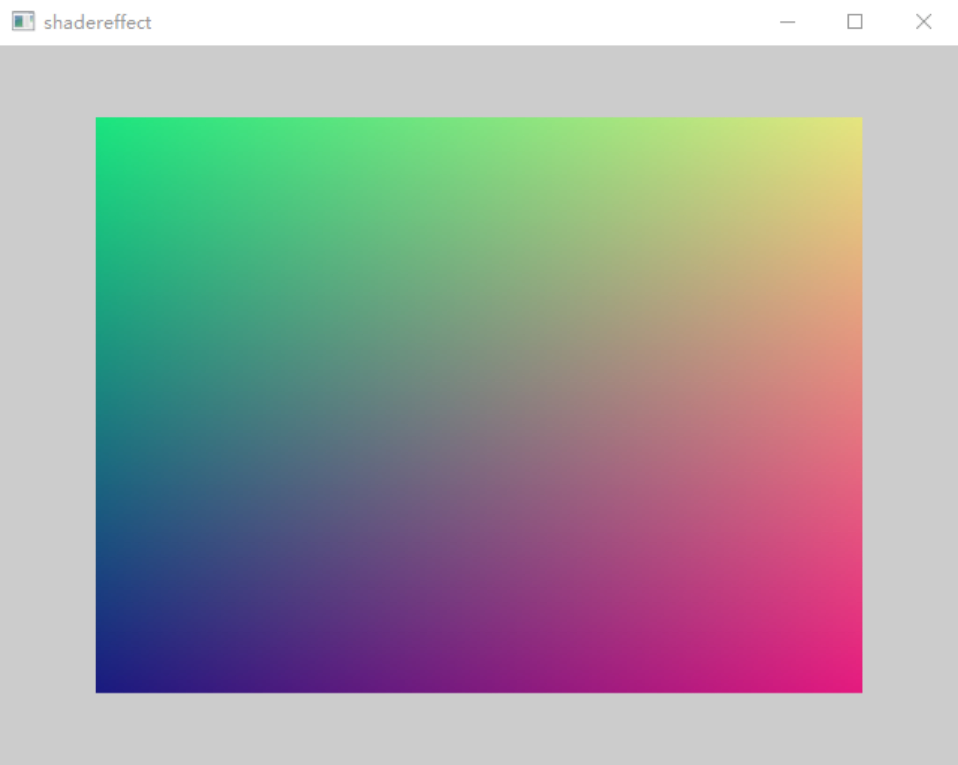
\includegraphics[width=0.95\textwidth]{the_book_image/p000008.pdf}} %图片路径
\caption{Qt Quick中使用着色器} %标题
\label{p000008} %索引
\end{figure}
%end图片


Qt Quick本身是使用OpenGL达成渲染的,
Qt Quick原生支持GLSL。

不过,考虑到硬件兼容性。目前在Qml中
使用GLSL,只支持
顶点着色器和片段着色器。

如果读者需要使用计算着色器、几何着色器或分型着色器,
读者需要使用C{\sourcefonttwo{}+}{\sourcefonttwo{}+}扩展Qml。

如\filesourcenumbernameone\ \ref{f000038}
第14\raisebox{0.16ex}{\sourcefonttwo\~{}}46行展示了如何使用“ShaderEffect”,在
Qt Quick中使用GLSL。

%\begin{spacing}{1.0}
\refstepcounter{filesourcenumber}\label{f000038}    %增加源代码编号
\FloatBarrier                                  %强制完成浮动体布局
\begin{thebookfilesourceone}[escapeinside={(*@}{@*)},
caption=GoodLuck,
title=\filesourcenumbernameone \thefilesourcenumber
]
/*shadereffect/main.qml*/
import QtQuick 2.9

Rectangle {

    width: 640;
    height: 480;
    color: Qt.rgba(0.8,0.8,0.8,1);

    Rectangle{
        anchors.centerIn: parent    ;
        width: parent.width * 0.8   ;
        height: parent.height * 0.8 ;
        ShaderEffect{
            anchors.fill: parent ;
            fragmentShader:"
/*片段着色器*/
#version 460

in vec2  qt_TexCoord0/*纹理坐标*/  ;
out vec4 fragColor   /*输出值*/    ;

uniform float qt_Opacity/*透明度*/ ;

void main() {
    vec4 varColor  = vec4( qt_TexCoord0.x ,  qt_TexCoord0.y , 0.5 , 1);
    fragColor = varColor * qt_Opacity;
}

"
            vertexShader :"
/*顶点着色器*/
#version 460

in vec4 qt_Vertex/*输入点坐标*/    ;
out vec2 qt_TexCoord0/*纹理坐标*/  ;

uniform mat4 qt_Matrix/*投影矩阵*/ ;

void main() {
    gl_Position = qt_Matrix * qt_Vertex;
    qt_TexCoord0 = gl_Position.xy*0.5 + 0.5 ;
}

"
        }
    }

}/*~Rectangle*/(*@\marginpar[\hfill\setlength\fboxsep{2pt}\fbox{\footnotesize{\kaishu\parbox{1em}{\setlength{\baselineskip}{2pt}\filesourcenumbernameone}}\footnotesize{\thefilesourcenumber}}]{\setlength\fboxsep{2pt}\fbox{\footnotesize{\kaishu\parbox{1em}{\setlength{\baselineskip}{2pt}\filesourcenumbernameone}}\footnotesize{\thefilesourcenumber}}}@*)\end{thebookfilesourceone}          %抄录环境
\addtocounter{lstlisting}{-1}   %sub lstlisting counter ...
%\end{spacing}
%main.qml

%%%%%%%%%%%%%%%%%%%%%%%%%%%%%%%%%%

使用“ShaderEffect”导入纹理是极为简单的。
读者只需要在“ShaderEffect”自定义
一个代表“Image”的属性,
在GLSL中就可以直接使用了。

如\filesourcenumbernameone\ \ref{f000039}
所示:

\begin{itemize}

\item 第14\raisebox{0.16ex}{\sourcefonttwo\~{}}18行定义了一个Image;
\item 第20行定在“ShaderEffect”中自定义了
一个名为的“source”属性,此属性指向Image对象;
\item 第30行在片段着色器中将
“source”属性作为一个纹理载入;

\end{itemize}

%begin图片
\begin{figure}[htb] %浮动体 here and top ...
%there must use marginnote ...
\marginnote{\setlength\fboxsep{2pt}\fbox{\footnotesize{\kaishu\figurename\,}\footnotesize{\ref{p000009}}}}\centering %中心对齐
\setlength\fboxsep{0pt}\fcolorbox[rgb]{0,0,0}{0.97,0.98,0.99}{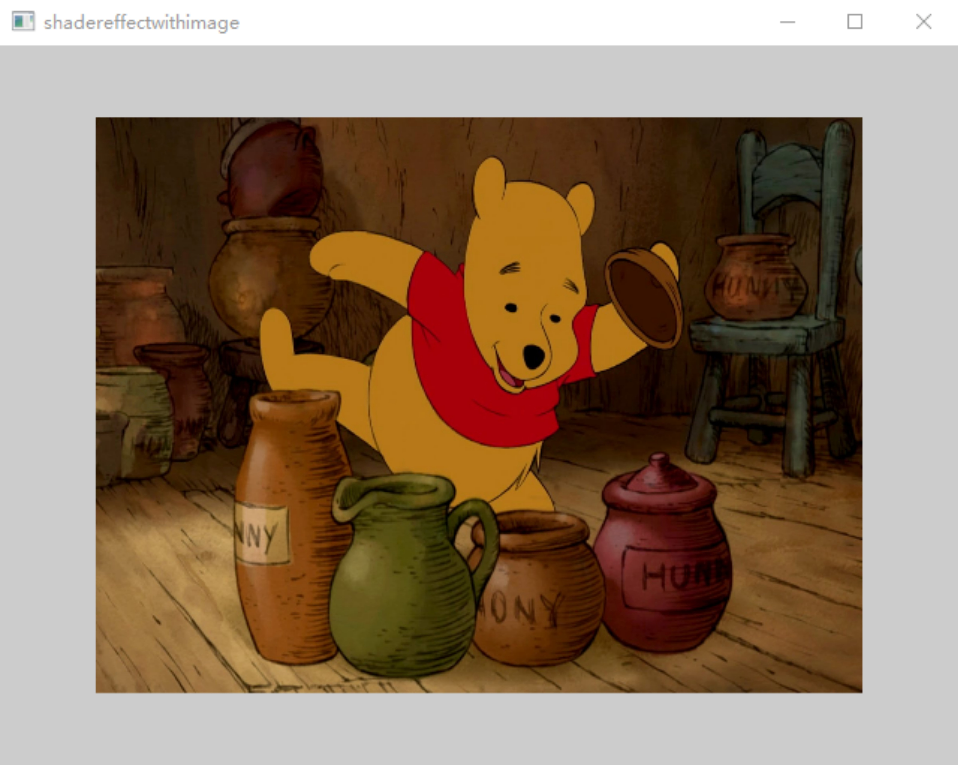
\includegraphics[width=0.95\textwidth]{the_book_image/p000009.pdf}} %图片路径
\caption{Qt Quick着色器中使用纹理} %标题
\label{p000009} %索引
\end{figure}
%end图片


%\begin{spacing}{1.0}
\refstepcounter{filesourcenumber}\label{f000039}    %增加源代码编号
\FloatBarrier                                  %强制完成浮动体布局
\begin{thebookfilesourceone}[escapeinside={(*@}{@*)},
caption=GoodLuck,
title=\filesourcenumbernameone \thefilesourcenumber
]
/*shadereffectwithimage/main.qml*/
import QtQuick 2.9

Rectangle {

    width: 640;
    height: 480;
    color: Qt.rgba(0.8,0.8,0.8,1);

    Rectangle{
        anchors.centerIn: parent    ;
        width: parent.width * 0.8   ;
        height: parent.height * 0.8 ;
        Image{
            id : idSourceImage;
            source: "0000.jpg";
            visible: false    ;
        }
        ShaderEffect{
            property variant source: idSourceImage/*the image...*/
            anchors.fill: parent ;
            fragmentShader:"
/*片段着色器*/
#version 460

in vec2 qt_TexCoord0;

out vec4 fragColor;

uniform sampler2D source/*the image...*/;
uniform float qt_Opacity;

void main() {
    fragColor = texture(source, qt_TexCoord0) * qt_Opacity;
}

"
            vertexShader :"
/*顶点着色器*/
#version 460

in vec4 qt_Vertex;
in vec2 qt_MultiTexCoord0;

out vec2 qt_TexCoord0;

uniform mat4 qt_Matrix;

void main() {
    qt_TexCoord0 = qt_MultiTexCoord0;
    gl_Position = qt_Matrix * qt_Vertex;
}

"
        }
    }

}/*~Rectangle*/(*@\marginpar[\hfill\setlength\fboxsep{2pt}\fbox{\footnotesize{\kaishu\parbox{1em}{\setlength{\baselineskip}{2pt}\filesourcenumbernameone}}\footnotesize{\thefilesourcenumber}}]{\setlength\fboxsep{2pt}\fbox{\footnotesize{\kaishu\parbox{1em}{\setlength{\baselineskip}{2pt}\filesourcenumbernameone}}\footnotesize{\thefilesourcenumber}}}@*)\end{thebookfilesourceone}          %抄录环境
\addtocounter{lstlisting}{-1}   %sub lstlisting counter ...
%\end{spacing}
%main.qml


% ______all_key_words
% the_book_chapter the_book_subsection the_book_subsubsection
% the_book_section the_book_image the_book_table
% the_book_file the_book_tree_file the_book_command_file
% littlelongworld tabbing ref
% figurename tablename filesourcenumbernameone
% treeindexnumbernameone commandnumbernameone footnote
% item itemize comment textbullet
% \hspace*{\parindent}







%使用XeLaTeX编译
%版权所有,翻版必究
%本文件由程序自动生成,任何修改将被覆盖
%2019 年 01 月 23 日





%使用XeLaTeX编译
%版权所有,翻版必究
%本文件由程序自动生成,任何修改将被覆盖
%2019 年 01 月 23 日




\FloatBarrier
\section{
使用C{\sourcefonttwo{}+}{\sourcefonttwo{}+}扩展Qt Quick
}\label{s100710}


读者可能认为使用Qt Quick只需要Qml足以,但不久读者就会失望。
即使退一步,希望Qt Quick可以满足绝大多数需求,这也是难以达成。

Qt Quick不是一种全面代替Qt C{\sourcefonttwo{}+}{\sourcefonttwo{}+}无所不包的解决方案。
Qt Quick只是导出Qt C{\sourcefonttwo{}+}{\sourcefonttwo{}+}的一套接口规范。

当读者面对一个具体的问题,在Qt Quick中无法找到现成的组件或者无法通过
简单修改现有Qt Quick组件达成目的时。使用Qt C{\sourcefonttwo{}+}{\sourcefonttwo{}+}自定义组件就势在必行。

\begin{itemize}

\item 如果所需的组件不需要几何逻辑,
比如实现一个本地文件监视器,那么只继承自QObject即可;

\item 如果所需的组件需要几何逻辑但无需渲染,
比如实现一个鼠标监视器,那么只需要继承自QQuickItem;

\item 如果所需的组件需要渲染,
那么需要继承自QQuickItem,并在构造函数中设置
QQuickItem::ItemHasContents标志位;

\item 如果希望使用QPainter实现渲染,
那么需要继承自QQuickPaintedItem是一个好的选择;

\item 如果仅需要一个简易的OpenGL离屏渲染环境,
那么继承自QQuickFramebufferObject是一个好的选择;

\end{itemize}

如\figurename\ \ref{p000010}
,列出了C{\sourcefonttwo{}+}{\sourcefonttwo{}+}导出Qt Quick基类继承关系图。

%begin图片
\begin{figure}[htb] %浮动体 here and top ...
%there must use marginnote ...
\marginnote{\setlength\fboxsep{2pt}\fbox{\footnotesize{\kaishu\figurename\,}\footnotesize{\ref{p000010}}}}\centering %中心对齐
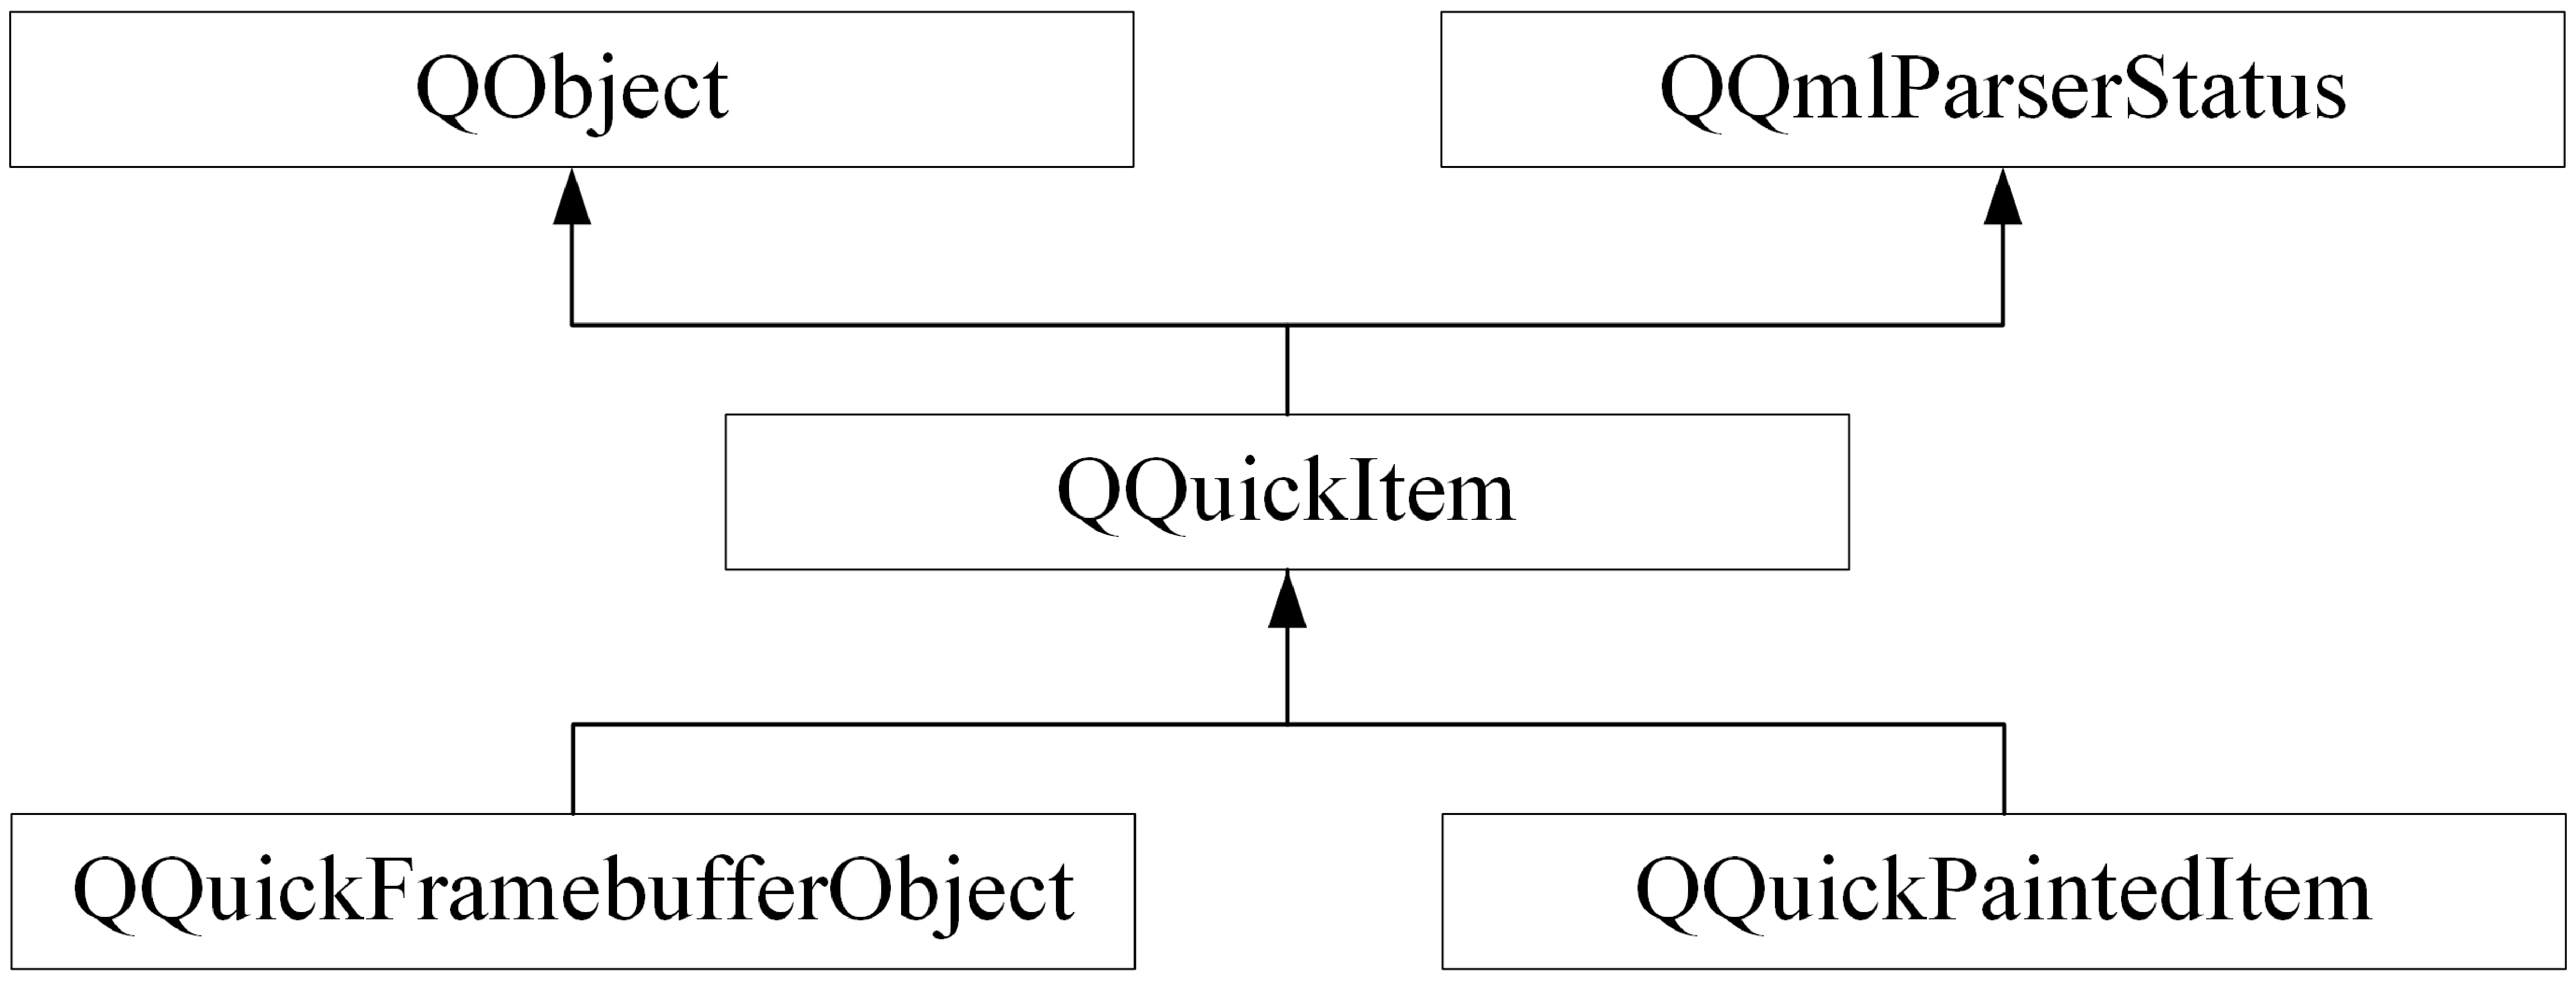
\includegraphics[width=0.95\textwidth]{the_book_image/p000010.eps} %图片路径
\caption{C{\sourcefonttwo{}+}{\sourcefonttwo{}+}导出Qt Quick所需基类} %标题
\label{p000010} %索引
\end{figure}
%end图片


本节展示直接使用C{\sourcefonttwo{}+}{\sourcefonttwo{}+}调用OpenGL绘制,并将其导出到Qt Quick。

本节示例位于目录“QtQmlBook/chapter01/directdrawbyopengl”。

%begin图片
\begin{figure}[htb] %浮动体 here and top ...
%there must use marginnote ...
\marginnote{\setlength\fboxsep{2pt}\fbox{\footnotesize{\kaishu\figurename\,}\footnotesize{\ref{p000011}}}}\centering %中心对齐
\setlength\fboxsep{0pt}\fbox{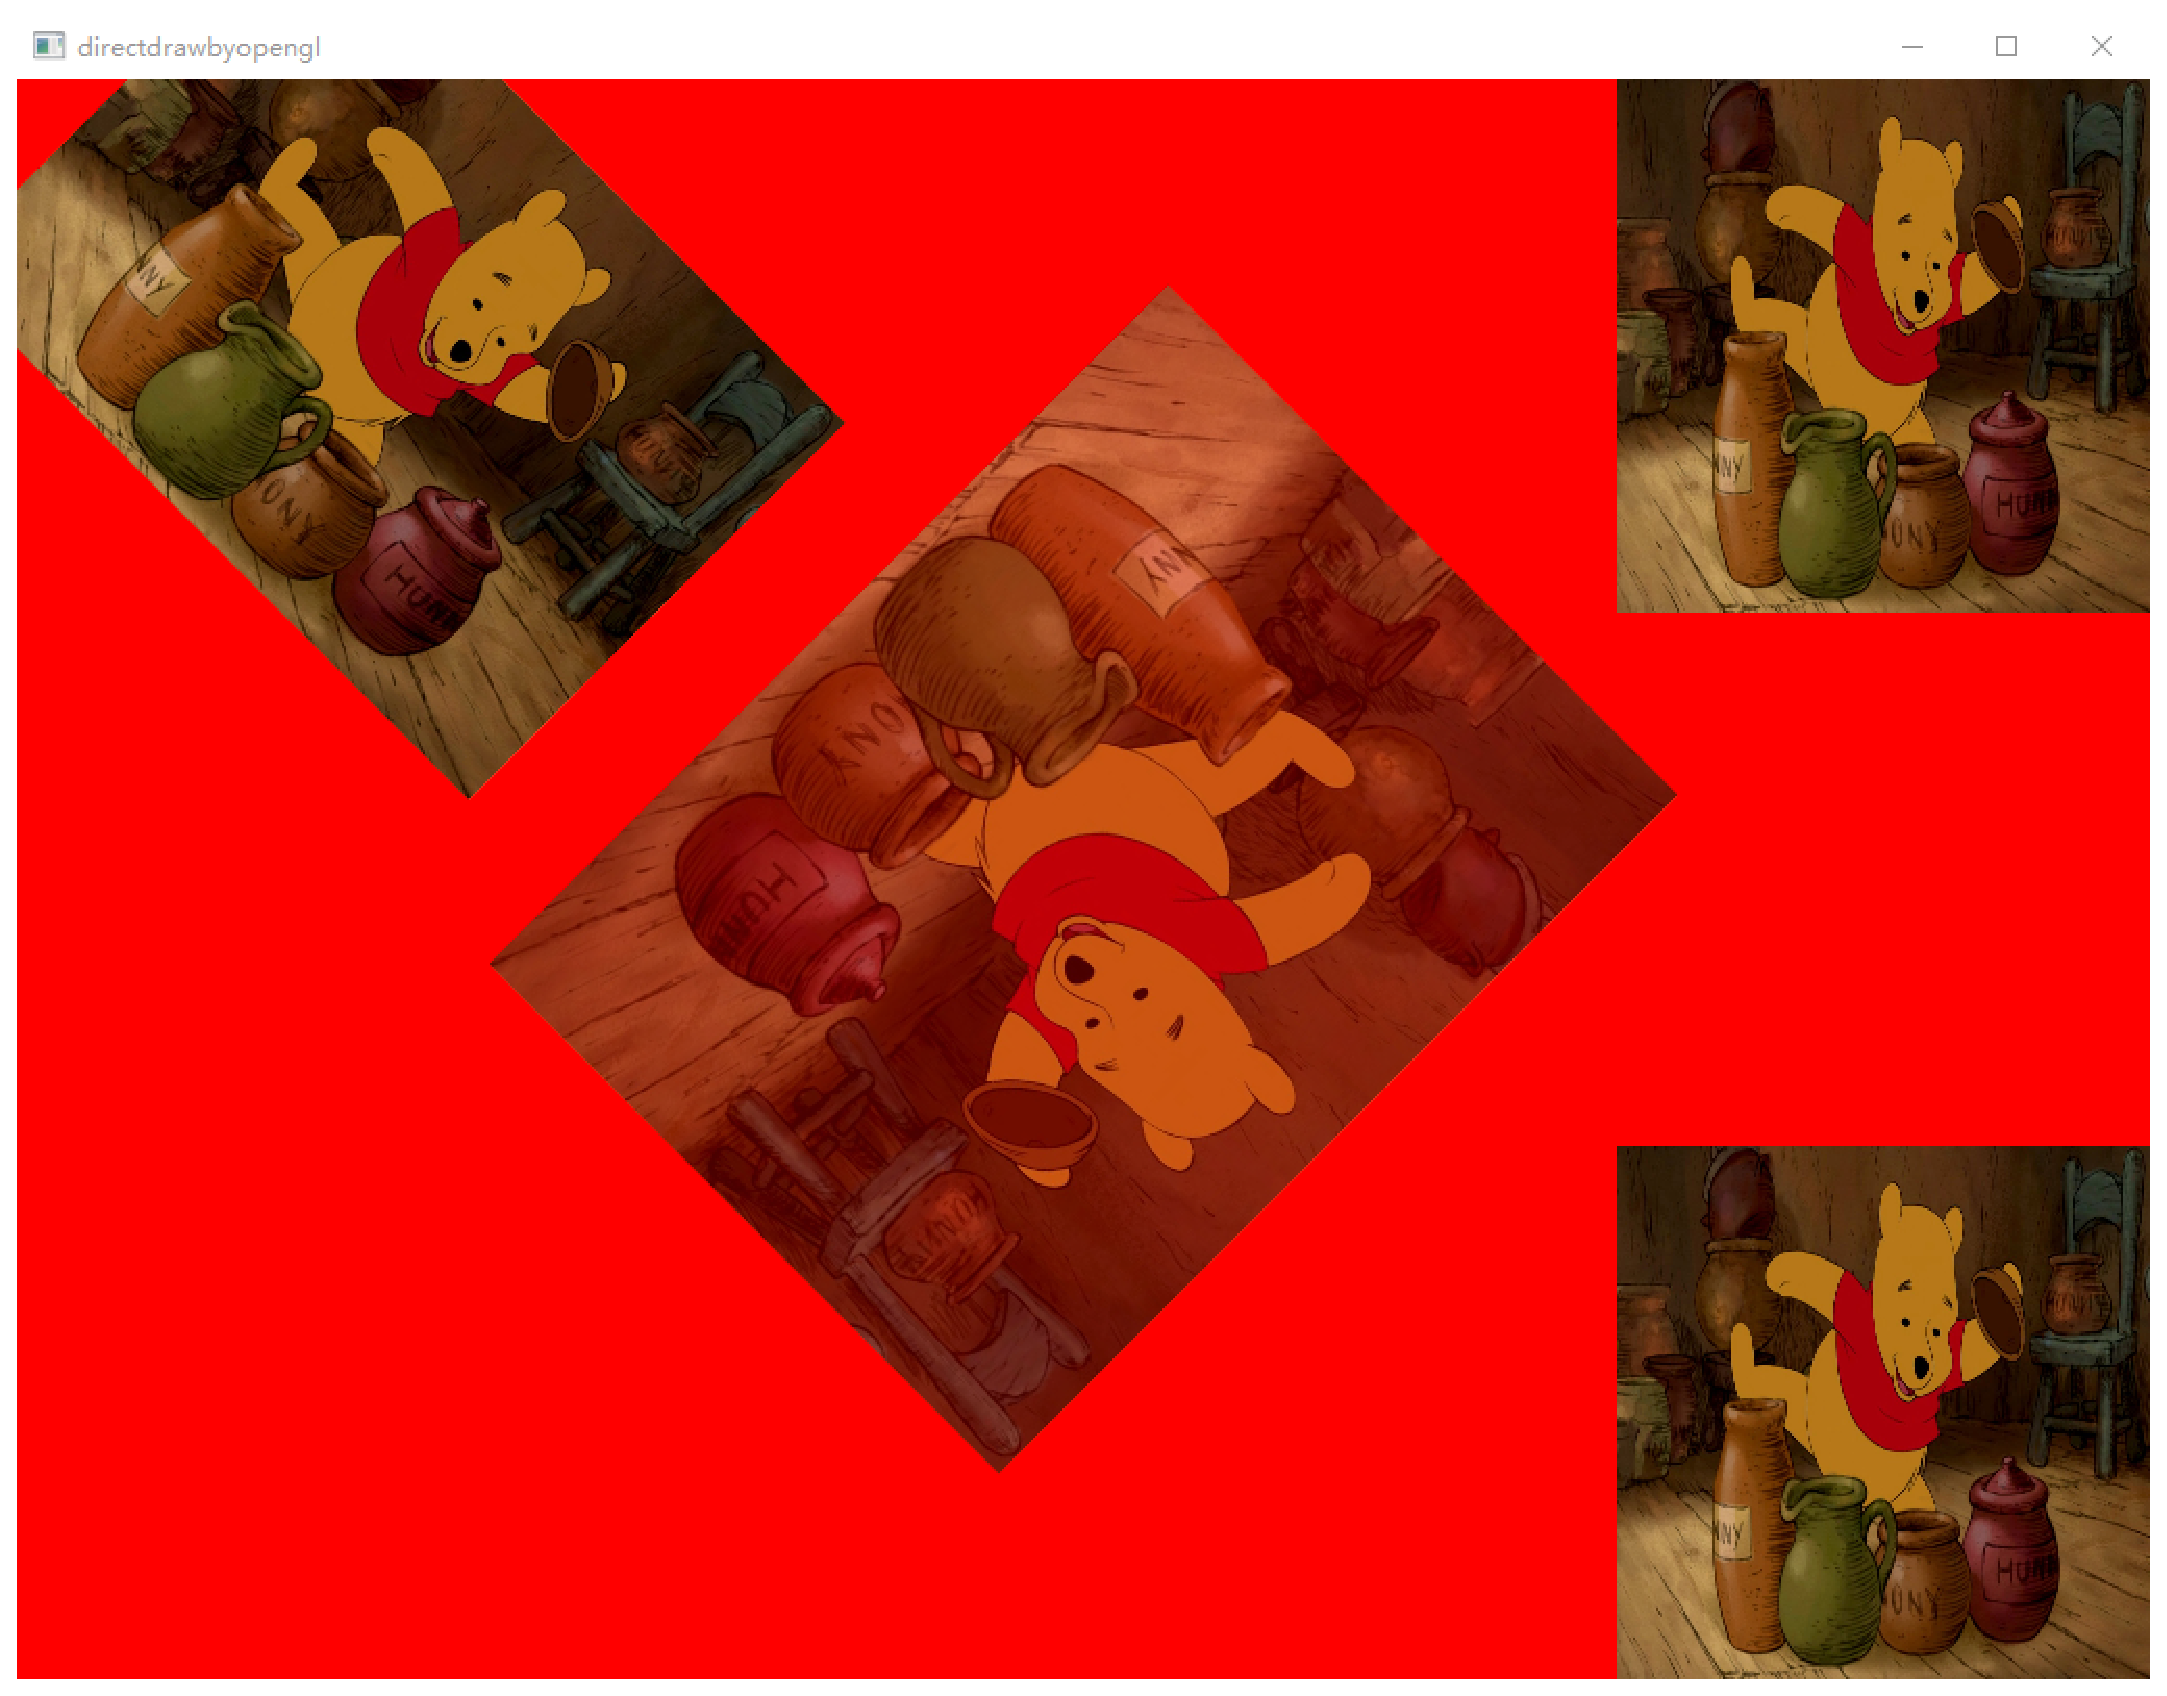
\includegraphics[width=0.95\textwidth]{the_book_image/p000011.eps}} %图片路径
\caption{直接使用OpenGL绘制} %标题
\label{p000011} %索引
\end{figure}
%end图片


先来看看Qt Quick代码,
如\filesourcenumbernameone\ \ref{f000042}。

%\begin{spacing}{1.0}
\refstepcounter{filesourcenumber}\label{f000042}    %增加源代码编号
\FloatBarrier                                  %强制完成浮动体布局
\begin{thebookfilesourceone}[escapeinside={(*@}{@*)},
caption=GoodLuck,
title=\filesourcenumbernameone \thefilesourcenumber
]
/*directdrawbyopengl/main.qml*/
import QtQuick 2.9
import sstd.quick 1.0

Rectangle{
    id : root_object
    objectName: "root_object";
    width: 1024 ;
    height: 768 ;
    color: Qt.rgba(1,0,0,1);

    DrawImageItemRaw {

        width: parent.width /2  ;
        height: parent.height /2;
        anchors.centerIn: parent;
        transformOrigin: Item.Center ;
        rawImage : Qt.resolvedUrl( "0000.jpg" );

        Timer{
            repeat: true;
            running: true;
            interval : 500 ;
            triggeredOnStart: true;
            onTriggered: {
                parent.rotation += 15 ;
                if(parent.rotation>360){
                    parent.rotation -= 360 ;
                }
                parent.opacity = Math.random() * 0.3 + 0.7 ;
                parent.scale = Math.random() * 0.3 + 0.7   ;
            }
        }

    }


    Component.onCompleted : {
        Qt.createQmlObject(
"
import QtQuick 2.9
import sstd.quick 1.0

DrawImageItemRaw {
    width: 256   ;
    height: 256  ;
    anchors.top: parent.top                 ;
    anchors.right : parent.right            ;
    rawImage : Qt.resolvedUrl( '0000.jpg' ) ;
}

" , root_object  ) ;
    }

}/*Rectangle*/(*@\marginpar[\hfill\setlength\fboxsep{2pt}\fbox{\footnotesize{\kaishu\parbox{1em}{\setlength{\baselineskip}{2pt}\filesourcenumbernameone}}\footnotesize{\thefilesourcenumber}}]{\setlength\fboxsep{2pt}\fbox{\footnotesize{\kaishu\parbox{1em}{\setlength{\baselineskip}{2pt}\filesourcenumbernameone}}\footnotesize{\thefilesourcenumber}}}@*)\end{thebookfilesourceone}          %抄录环境
\addtocounter{lstlisting}{-1}   %sub lstlisting counter ...
%\end{spacing}


\begin{itemize}

\item 第3行引入自定义模块。
其对应的C{\sourcefonttwo{}+}{\sourcefonttwo{}+}代码如\filesourcenumbernameone\ \ref{f000043}:
%\begin{spacing}{1.0}
\refstepcounter{filesourcenumber}\label{f000043}    %增加源代码编号
\FloatBarrier                                  %强制完成浮动体布局
\begin{thebookfilesourceone}[escapeinside={(*@}{@*)},
caption=GoodLuck,
title=\filesourcenumbernameone \thefilesourcenumber
]
static inline void register_this() {
    qmlRegisterType<DrawImageItem>(
        "sstd.quick",
        1, 0,
        "DrawImageItemRaw");
}
Q_COREAPP_STARTUP_FUNCTION(register_this)(*@\marginpar[\hfill\setlength\fboxsep{2pt}\fbox{\footnotesize{\kaishu\parbox{1em}{\setlength{\baselineskip}{2pt}\filesourcenumbernameone}}\footnotesize{\thefilesourcenumber}}]{\setlength\fboxsep{2pt}\fbox{\footnotesize{\kaishu\parbox{1em}{\setlength{\baselineskip}{2pt}\filesourcenumbernameone}}\footnotesize{\thefilesourcenumber}}}@*)\end{thebookfilesourceone}          %抄录环境
\addtocounter{lstlisting}{-1}   %sub lstlisting counter ...
%\end{spacing}


本节的示例依然是静态加载,
实际上Qt Quick也支持以插件的形式动态加载组件。

\item 第12\raisebox{0.16ex}{\sourcefonttwo\~{}}35行演示了如何使用
自定义模块中的类“DrawImageItemRaw”。

使用C{\sourcefonttwo{}+}{\sourcefonttwo{}+}自定义的类与Qt Quick原生元素没有什么不同。
信号槽、平移、旋转、缩放……

不难发现,
使用Qt Quick可以将一切从极高的抽象层上
迅速的组装起来。

\item 第38\raisebox{0.16ex}{\sourcefonttwo\~{}}53行演示了直接在
Qt Quick里面编译Qt Quick源码并以此创建对象。

正如读者所见,
Qt Quick拥有脚本语言的所有特性,
并可以与Qt C{\sourcefonttwo{}+}{\sourcefonttwo{}+}无缝通信。

\end{itemize}

%\begin{spacing}{1.0}
\refstepcounter{filesourcenumber}\label{f000044}    %增加源代码编号
\FloatBarrier                                  %强制完成浮动体布局
\begin{thebookfilesourceone}[escapeinside={(*@}{@*)},
caption=GoodLuck,
title=\filesourcenumbernameone \thefilesourcenumber
]
/*directdrawbyopengl/main.cpp*/
#include <sstd_qt_and_qml_library.hpp>
#include "DrawImageItem.hpp"

int main(int argc, char ** argv) {

    /*初始化程序*/
    auto varApp = sstd_make_unique< sstd::Application >(argc, argv);
    /*初始化Qml/Quick引擎*/
    auto varWindow = sstd_make_unique< sstd::DefaultRoowWindow >();
    {
        /*获得Qml文件绝对路径*/
        auto varFullFileName = sstd::getLocalFileFullPath(
            QStringLiteral("myqml/directdrawbyopengl/main.qml"));

        /*加载Qml文件*/
        varWindow->load(varFullFileName);
        /*检查并报错*/
        if (varWindow->status() != sstd::LoadState::Ready) {
            qWarning() << QStringLiteral("can not load : ")
            << varFullFileName;
            return -1;
        }

    }

    varWindow->show();

    {
        /*运行时由C++端添加对象*/
        auto varRootObject = varWindow->getRootObject();
        assert(varRootObject);
        assert(varRootObject->objectName() == QStringLiteral("root_object"));
        auto varItem = sstd_new<DrawImageItem>();
        varItem->setParent(varRootObject);
        const auto varImage = QImage(sstd::getLocalFileFullFilePath(
            QStringLiteral("myqml/directdrawbyopengl/0000.jpg")));
        varItem->setImage(varImage);
        varItem->setWidth(360);
        varItem->setHeight(256);
        varItem->setTransformOrigin(QQuickItem::Center);
        varItem->setRotation(45);
        varItem->setParentItem(varRootObject);
    }

    {
        /*运行时由C++编译QML对象*/
        const auto varQmlCode = u8R"+++(

import QtQuick 2.9
import sstd.quick 1.0

DrawImageItemRaw {

    width: 256                             ;
    height: 256                            ;
    rawImage : Qt.resolvedUrl( "0000.jpg" );
    anchors.bottom: parent.bottom          ;
    anchors.right : parent.right           ;

}

)+++"sv;

        QQmlComponent varComponent{ varWindow->getEngine() };
        auto varContex = QQmlEngine::contextForObject( varWindow->getRootObject() );
        varComponent.setData(
            QByteArray( varQmlCode.data(),static_cast<int>(varQmlCode.size()) ),
            varContex->baseUrl()
        );
        auto varObject = sstd_runtime_cast<DrawImageItem>(
            varComponent.beginCreate( varContex ) );
        assert(varObject);
        varObject->setParent(varWindow->getRootObject());
        varObject->setParentItem(varWindow->getRootObject());
        varComponent.completeCreate();

    }

    return varApp->exec();

}(*@\marginpar[\hfill\setlength\fboxsep{2pt}\fbox{\footnotesize{\kaishu\parbox{1em}{\setlength{\baselineskip}{2pt}\filesourcenumbernameone}}\footnotesize{\thefilesourcenumber}}]{\setlength\fboxsep{2pt}\fbox{\footnotesize{\kaishu\parbox{1em}{\setlength{\baselineskip}{2pt}\filesourcenumbernameone}}\footnotesize{\thefilesourcenumber}}}@*)\end{thebookfilesourceone}          %抄录环境
\addtocounter{lstlisting}{-1}   %sub lstlisting counter ...
%\end{spacing}









%使用XeLaTeX编译
%版权所有,翻版必究
%本文件由程序自动生成,任何修改将被覆盖
%2019 年 01 月 23 日






















%使用XeLaTeX编译
%版权所有,翻版必究
%本文件由程序自动生成,任何修改将被覆盖
%2019 年 01 月 23 日



   %第一章

%使用xelatex编译
%版权所有,翻版必究
%本文件由程序自动生成,任何修改将被覆盖
%2019 年 01 月 09 日




%\FloatBarrier
\cleardoublepage
\chapter{
Qt Quick基础
}\label{c000011}



















%使用xelatex编译
%版权所有,翻版必究
%本文件由程序自动生成,任何修改将被覆盖
%2019 年 01 月 09 日



   %第二章
%使用xelatex编译
%版权所有,翻版必究
%本文件由程序自动生成,任何修改将被覆盖





\cleardoublepage
\chapter{
从C{\sourcefontone{}+}{\sourcefontone{}+}扩展Qt Quick
}\label{c000012}

















%使用xelatex编译
%版权所有,翻版必究
%本文件由程序自动生成,任何修改将被覆盖



   %第三章

%使用XeLaTeX编译
%版权所有,翻版必究
%本文件由程序自动生成,任何修改将被覆盖
%2019 年 01 月 23 日




%\FloatBarrier
\cleardoublepage
\chapter{
状态机及动画
}\label{c000013}



















%使用XeLaTeX编译
%版权所有,翻版必究
%本文件由程序自动生成,任何修改将被覆盖
%2019 年 01 月 23 日



   %第四章
%使用xelatex编译
%版权所有,翻版必究
%本文件由程序自动生成,任何修改将被覆盖





\cleardoublepage
\chapter{
粒子系统
}


















%使用xelatex编译
%版权所有,翻版必究
%本文件由程序自动生成,任何修改将被覆盖



   %第五章
%使用xelatex编译
%版权所有,翻版必究
%本文件由程序自动生成,任何修改将被覆盖




%\FloatBarrier
\cleardoublepage
\chapter{
特效
}\label{c000015}


















%使用xelatex编译
%版权所有,翻版必究
%本文件由程序自动生成,任何修改将被覆盖



   %第六章

%使用XeLaTeX编译
%版权所有,翻版必究
%本文件由程序自动生成,任何修改将被覆盖
%2019 年 01 月 23 日




%\FloatBarrier
\cleardoublepage
\chapter{
多媒体
}\label{c000016}



% ______all_key_words
% the_book_chapter the_book_subsection the_book_subsubsection
% the_book_section the_book_image the_book_table
% the_book_file the_book_tree_file the_book_command_file
% littlelongworld tabbing ref
% figurename tablename filesourcenumbernameone
% treeindexnumbernameone commandnumbernameone footnote 
% item itemize comment textbullet
% \hspace*{\parindent}







%使用XeLaTeX编译
%版权所有,翻版必究
%本文件由程序自动生成,任何修改将被覆盖
%2019 年 01 月 23 日



   %第七章

%使用XeLaTeX编译
%版权所有,翻版必究
%本文件由程序自动生成,任何修改将被覆盖
%2019 年 01 月 23 日




%\FloatBarrier
\cleardoublepage
\chapter{
富文本及图表
}\label{c000017}






%使用XeLaTeX编译
%版权所有,翻版必究
%本文件由程序自动生成,任何修改将被覆盖
%2019 年 01 月 23 日






%第一个charts...

%使用XeLaTeX编译
%版权所有,翻版必究
%本文件由程序自动生成,任何修改将被覆盖
%2019 年 01 月 23 日




\FloatBarrier
\section{
曲线图导引
}\label{c000017s01}





















% ______all_key_words
% the_book_chapter the_book_subsection the_book_subsubsection
% the_book_section the_book_image the_book_table
% the_book_file the_book_tree_file the_book_command_file
% littlelongworld tabbing ref
% figurename tablename filesourcenumbernameone
% treeindexnumbernameone commandnumbernameone footnote 
% item itemize comment textbullet







%使用XeLaTeX编译
%版权所有,翻版必究
%本文件由程序自动生成,任何修改将被覆盖
%2019 年 01 月 23 日








% ______all_key_words
% the_book_chapter the_book_subsection the_book_subsubsection
% the_book_section the_book_image the_book_table
% the_book_file the_book_tree_file the_book_command_file
% littlelongworld tabbing ref
% figurename tablename filesourcenumbernameone
% treeindexnumbernameone commandnumbernameone footnote 
% item itemize comment textbullet
% \hspace*{\parindent}







%使用XeLaTeX编译
%版权所有,翻版必究
%本文件由程序自动生成,任何修改将被覆盖
%2019 年 01 月 23 日








% ______all_key_words
% the_book_chapter the_book_subsection the_book_subsubsection
% the_book_section the_book_image the_book_table
% the_book_file the_book_tree_file the_book_command_file
% littlelongworld tabbing ref
% figurename tablename filesourcenumbernameone
% treeindexnumbernameone commandnumbernameone footnote
% item itemize comment textbullet
% \hspace*{\parindent}
% FloatBarrier







%使用XeLaTeX编译
%版权所有,翻版必究
%本文件由程序自动生成,任何修改将被覆盖
%2019 年 01 月 23 日
   %第八章
%使用xelatex编译
%版权所有,翻版必究
%本文件由程序自动生成,任何修改将被覆盖




%\FloatBarrier
\cleardoublepage
\chapter{
控件
}\label{c000018}


















%使用xelatex编译
%版权所有,翻版必究
%本文件由程序自动生成,任何修改将被覆盖



   %第九章

%使用XeLaTeX编译
%版权所有,翻版必究
%本文件由程序自动生成,任何修改将被覆盖
%2019 年 01 月 23 日




%\FloatBarrier
\cleardoublepage
\chapter{
模型视图
}\label{c000019}


Qt Widgets中的模型视图非常难用。

在Qt Widgets中的模型视图
架构中,每一个单独的项不是
一个单独的QWidget。
而是通过QPainter进行绘制,
并通过一些函数响应鼠标键盘事件。

这就造成了如果读者想
实现一些复杂的动态效果就
不得不自己实现一个超级复杂
的状态机系统。

而在Qt Quick中一切可视元素都是一致的。

视图是QQuickItem的子类,
视图中的每一项也是QQuickItem的子类。
在Qt Quick体系中一切都是对象!

读者可以使用Qt Quick的模型视图架构,
将数据与渲染和控制完全分离。
而且,
这种实现是极其高效的,
即使模型拥有高达数亿元素。
Qt Quick的模型视图架构也可以快速
布局并迅速渲染。











%使用XeLaTeX编译
%版权所有,翻版必究
%本文件由程序自动生成,任何修改将被覆盖
%2019 年 01 月 23 日



   %第十章

\cleardoublepage                              %增加空白页
\CTEXsetup[format={\bfseries\raggedright}]{section} %section左对齐
\setcounter{secnumdepth}{-2}                  %暂停编号,但加入目录
\chapter{附录}
\begin{multicols}{3}
\section{图片索引}

%使用XeLaTeX编译
%版权所有,翻版必究
%本文件由程序自动生成,任何修改将被覆盖
%2019 年 01 月 23 日



\noindent\figurename\ \ref{p000000},\ \pageref{p000000}

\noindent\figurename\ \ref{p000001},\ \pageref{p000001}

\noindent\figurename\ \ref{p000002},\ \pageref{p000002}

\noindent\figurename\ \ref{p000003},\ \pageref{p000003}

\noindent\figurename\ \ref{p000004},\ \pageref{p000004}

\noindent\figurename\ \ref{p000005},\ \pageref{p000005}

\noindent\figurename\ \ref{p000006},\ \pageref{p000006}

\noindent\figurename\ \ref{p000007},\ \pageref{p000007}

\noindent\figurename\ \ref{p000008},\ \pageref{p000008}

\noindent\figurename\ \ref{p000009},\ \pageref{p000009}

\noindent\figurename\ \ref{p000010},\ \pageref{p000010}

\noindent\figurename\ \ref{p000011},\ \pageref{p000011}

\noindent\figurename\ \ref{p000043},\ \pageref{p000043}

\noindent\figurename\ \ref{p000012},\ \pageref{p000012}

\noindent\figurename\ \ref{p000018},\ \pageref{p000018}

\noindent\figurename\ \ref{p000019},\ \pageref{p000019}

\noindent\figurename\ \ref{p000020},\ \pageref{p000020}

\noindent\figurename\ \ref{p000021},\ \pageref{p000021}

\noindent\figurename\ \ref{p000022},\ \pageref{p000022}

\noindent\figurename\ \ref{p000023},\ \pageref{p000023}

\noindent\figurename\ \ref{p000024},\ \pageref{p000024}

\noindent\figurename\ \ref{p000025},\ \pageref{p000025}

\noindent\figurename\ \ref{p000026},\ \pageref{p000026}

\noindent\figurename\ \ref{p000027},\ \pageref{p000027}

\noindent\figurename\ \ref{p000028},\ \pageref{p000028}

\noindent\figurename\ \ref{p000029},\ \pageref{p000029}

\noindent\figurename\ \ref{p000030},\ \pageref{p000030}

\noindent\figurename\ \ref{p000031},\ \pageref{p000031}

\noindent\figurename\ \ref{p000032},\ \pageref{p000032}

\noindent\figurename\ \ref{p000033},\ \pageref{p000033}

\noindent\figurename\ \ref{p000034},\ \pageref{p000034}

\noindent\figurename\ \ref{p000035},\ \pageref{p000035}

\noindent\figurename\ \ref{p000036},\ \pageref{p000036}

\noindent\figurename\ \ref{p000037},\ \pageref{p000037}

\noindent\figurename\ \ref{p000038},\ \pageref{p000038}

\noindent\figurename\ \ref{p000039},\ \pageref{p000039}

\noindent\figurename\ \ref{p000040},\ \pageref{p000040}

\noindent\figurename\ \ref{p000041},\ \pageref{p000041}

\noindent\figurename\ \ref{p000042},\ \pageref{p000042}






%使用XeLaTeX编译
%版权所有,翻版必究
%本文件由程序自动生成,任何修改将被覆盖
%2019 年 01 月 23 日



                       %图片索引目录
\section{表格索引}

%使用XeLaTeX编译
%版权所有,翻版必究
%本文件由程序自动生成,任何修改将被覆盖
%2019 年 01 月 23 日



\noindent\tablename\ \ref{tb000000},\ \pageref{tb000000}%tb000000






%使用XeLaTeX编译
%版权所有,翻版必究
%本文件由程序自动生成,任何修改将被覆盖
%2019 年 01 月 23 日



                        %表格索引目录
\section{源码索引}

%使用XeLaTeX编译
%版权所有,翻版必究
%本文件由程序自动生成,任何修改将被覆盖
%2019 年 01 月 23 日



\noindent\filesourcenumbernameone\ \ref{f000041},\ \pageref{f000041}%f000041

\noindent\filesourcenumbernameone\ \ref{f000040},\ \pageref{f000040}%f000040

\noindent\filesourcenumbernameone\ \ref{f000002},\ \pageref{f000002}%f000002

\noindent\filesourcenumbernameone\ \ref{f000003},\ \pageref{f000003}%f000003

\noindent\filesourcenumbernameone\ \ref{f00000d},\ \pageref{f00000d}%f00000d

\noindent\filesourcenumbernameone\ \ref{f000010},\ \pageref{f000010}%f000010

\noindent\filesourcenumbernameone\ \ref{f000016},\ \pageref{f000016}%f000016

\noindent\filesourcenumbernameone\ \ref{f000011},\ \pageref{f000011}%f000011

\noindent\filesourcenumbernameone\ \ref{f000012},\ \pageref{f000012}%f000012

\noindent\filesourcenumbernameone\ \ref{f000014},\ \pageref{f000014}%f000014

\noindent\filesourcenumbernameone\ \ref{f000013},\ \pageref{f000013}%f000013

\noindent\filesourcenumbernameone\ \ref{f000015},\ \pageref{f000015}%f000015

\noindent\filesourcenumbernameone\ \ref{f000004},\ \pageref{f000004}%f000004

\noindent\filesourcenumbernameone\ \ref{f000005},\ \pageref{f000005}%f000005

\noindent\filesourcenumbernameone\ \ref{f000008},\ \pageref{f000008}%f000008

\noindent\filesourcenumbernameone\ \ref{f000009},\ \pageref{f000009}%f000009

\noindent\filesourcenumbernameone\ \ref{f000006},\ \pageref{f000006}%f000006

\noindent\filesourcenumbernameone\ \ref{f000007},\ \pageref{f000007}%f000007

\noindent\filesourcenumbernameone\ \ref{f00000b},\ \pageref{f00000b}%f00000b

\noindent\filesourcenumbernameone\ \ref{f00000c},\ \pageref{f00000c}%f00000c

\noindent\filesourcenumbernameone\ \ref{f00000a},\ \pageref{f00000a}%f00000a

\noindent\filesourcenumbernameone\ \ref{f000017},\ \pageref{f000017}%f000017

\noindent\filesourcenumbernameone\ \ref{f000018},\ \pageref{f000018}%f000018

\noindent\filesourcenumbernameone\ \ref{f000019},\ \pageref{f000019}%f000019

\noindent\filesourcenumbernameone\ \ref{f000026},\ \pageref{f000026}%f000026

\noindent\filesourcenumbernameone\ \ref{f000027},\ \pageref{f000027}%f000027

\noindent\filesourcenumbernameone\ \ref{f000028},\ \pageref{f000028}%f000028

\noindent\filesourcenumbernameone\ \ref{f000029},\ \pageref{f000029}%f000029

\noindent\filesourcenumbernameone\ \ref{f00002u},\ \pageref{f00002u}%f00002u

\noindent\filesourcenumbernameone\ \ref{f000020},\ \pageref{f000020}%f000020

\noindent\filesourcenumbernameone\ \ref{f000023},\ \pageref{f000023}%f000023

\noindent\filesourcenumbernameone\ \ref{f000021},\ \pageref{f000021}%f000021

\noindent\filesourcenumbernameone\ \ref{f000024},\ \pageref{f000024}%f000024

\noindent\filesourcenumbernameone\ \ref{f000022},\ \pageref{f000022}%f000022

\noindent\filesourcenumbernameone\ \ref{f000025},\ \pageref{f000025}%f000025

\noindent\filesourcenumbernameone\ \ref{f000030},\ \pageref{f000030}%f000030

\noindent\filesourcenumbernameone\ \ref{f000031},\ \pageref{f000031}%f000031

\noindent\filesourcenumbernameone\ \ref{f000034},\ \pageref{f000034}%f000034

\noindent\filesourcenumbernameone\ \ref{f000032},\ \pageref{f000032}%f000032

\noindent\filesourcenumbernameone\ \ref{f000033},\ \pageref{f000033}%f000033

\noindent\filesourcenumbernameone\ \ref{f000035},\ \pageref{f000035}%f000035

\noindent\filesourcenumbernameone\ \ref{f000037},\ \pageref{f000037}%f000037

\noindent\filesourcenumbernameone\ \ref{f000036},\ \pageref{f000036}%f000036

\noindent\filesourcenumbernameone\ \ref{f000038},\ \pageref{f000038}%f000038

\noindent\filesourcenumbernameone\ \ref{f000039},\ \pageref{f000039}%f000039

\noindent\filesourcenumbernameone\ \ref{f000042},\ \pageref{f000042}%f000042

\noindent\filesourcenumbernameone\ \ref{f000043},\ \pageref{f000043}%f000043

\noindent\filesourcenumbernameone\ \ref{f000044},\ \pageref{f000044}%f000044

\noindent\filesourcenumbernameone\ \ref{f000051},\ \pageref{f000051}%f000051

\noindent\filesourcenumbernameone\ \ref{f000052},\ \pageref{f000052}%f000052

\noindent\filesourcenumbernameone\ \ref{f000050},\ \pageref{f000050}%f000050

\noindent\filesourcenumbernameone\ \ref{f000077},\ \pageref{f000077}%f000077

\noindent\filesourcenumbernameone\ \ref{f000053},\ \pageref{f000053}%f000053

\noindent\filesourcenumbernameone\ \ref{f000054},\ \pageref{f000054}%f000054

\noindent\filesourcenumbernameone\ \ref{f000055},\ \pageref{f000055}%f000055

\noindent\filesourcenumbernameone\ \ref{f000056},\ \pageref{f000056}%f000056

\noindent\filesourcenumbernameone\ \ref{f000057},\ \pageref{f000057}%f000057

\noindent\filesourcenumbernameone\ \ref{f000058},\ \pageref{f000058}%f000058

\noindent\filesourcenumbernameone\ \ref{f000059},\ \pageref{f000059}%f000059

\noindent\filesourcenumbernameone\ \ref{f000060},\ \pageref{f000060}%f000060

\noindent\filesourcenumbernameone\ \ref{f000061},\ \pageref{f000061}%f000061

\noindent\filesourcenumbernameone\ \ref{f000062},\ \pageref{f000062}%f000062

\noindent\filesourcenumbernameone\ \ref{f000063},\ \pageref{f000063}%f000063

\noindent\filesourcenumbernameone\ \ref{f000064},\ \pageref{f000064}%f000064

\noindent\filesourcenumbernameone\ \ref{f000065},\ \pageref{f000065}%f000065

\noindent\filesourcenumbernameone\ \ref{f000066},\ \pageref{f000066}%f000066

\noindent\filesourcenumbernameone\ \ref{f000067},\ \pageref{f000067}%f000067

\noindent\filesourcenumbernameone\ \ref{f000068},\ \pageref{f000068}%f000068

\noindent\filesourcenumbernameone\ \ref{f000069},\ \pageref{f000069}%f000069

\noindent\filesourcenumbernameone\ \ref{f000070},\ \pageref{f000070}%f000070

\noindent\filesourcenumbernameone\ \ref{f000071},\ \pageref{f000071}%f000071

\noindent\filesourcenumbernameone\ \ref{f000072},\ \pageref{f000072}%f000072

\noindent\filesourcenumbernameone\ \ref{f000073},\ \pageref{f000073}%f000073

\noindent\filesourcenumbernameone\ \ref{f000074},\ \pageref{f000074}%f000074

\noindent\filesourcenumbernameone\ \ref{f000075},\ \pageref{f000075}%f000075

\noindent\filesourcenumbernameone\ \ref{f000076},\ \pageref{f000076}%f000076






%使用XeLaTeX编译
%版权所有,翻版必究
%本文件由程序自动生成,任何修改将被覆盖
%2019 年 01 月 23 日



                       %源码索引目录
\section{命令索引}

%使用XeLaTeX编译
%版权所有,翻版必究
%本文件由程序自动生成,任何修改将被覆盖
%2019 年 01 月 23 日



\noindent\commandnumbernameone\ \ref{command000002s02}\dotfill\pageref{command000002s02}%command000002s02

\noindent\commandnumbernameone\ \ref{command000002s01}\dotfill\pageref{command000002s01}%command000002s01

\noindent\commandnumbernameone\ \ref{command000000}\dotfill\pageref{command000000}%command000000

\noindent\commandnumbernameone\ \ref{command000001}\dotfill\pageref{command000001}%command000001

\noindent\commandnumbernameone\ \ref{command000002}\dotfill\pageref{command000002}%command000002

\noindent\commandnumbernameone\ \ref{command000003}\dotfill\pageref{command000003}%command000003






%使用XeLaTeX编译
%版权所有,翻版必究
%本文件由程序自动生成,任何修改将被覆盖
%2019 年 01 月 23 日
                %命令索引目录
\section{路径索引}

%使用XeLaTeX编译
%版权所有,翻版必究
%本文件由程序自动生成,任何修改将被覆盖
%2019 年 01 月 23 日



\noindent\treeindexnumbernameone\ \ref{d000001}\dotfill\pageref{d000001}%d000001

\noindent\treeindexnumbernameone\ \ref{d000000}\dotfill\pageref{d000000}%d000000

\noindent\treeindexnumbernameone\ \ref{d000002}\dotfill\pageref{d000002}%d000002






%使用XeLaTeX编译
%版权所有,翻版必究
%本文件由程序自动生成,任何修改将被覆盖
%2019 年 01 月 23 日
                %目录树索引目录
\end{multicols}

\backmatter
%%%%%%%%%%%%%%%%%%%%%%%%%%%%%%%%%%%%%%%%%%%%%%%%%%%%%%%%%%%%%%%%%%%%%%%%%%%%%

\end{document}

% \enlargethispage{1cm}
% http://www.ctex.org/documents/latex/graphics/node2.html
% https://www.jianshu.com/p/b1751078e28e
% \tiny
% \scriptsize
% \footnotesize
% \small
% \normalsize
% \large
% \Large
% \LARGE
% \huge
% \Huge




% ______all_key_words
% the_book_chapter the_book_subsection the_book_subsubsection
% the_book_section the_book_image the_book_table
% the_book_file the_book_tree_file the_book_command_file
% littlelongworld tabbing ref
% figurename tablename filesourcenumbernameone
% treeindexnumbernameone commandnumbernameone footnote
% item itemize comment textbullet
% \hspace*{\parindent}
% FloatBarrier







%使用XeLaTeX编译
%版权所有,翻版必究
%本文件由程序自动生成,任何修改将被覆盖
%2019 年 01 月 23 日



